\documentclass[]{article}
\usepackage{lmodern}
\usepackage{amssymb,amsmath}
\usepackage{ifxetex,ifluatex}
\usepackage{fixltx2e} % provides \textsubscript
\ifnum 0\ifxetex 1\fi\ifluatex 1\fi=0 % if pdftex
  \usepackage[T1]{fontenc}
  \usepackage[utf8]{inputenc}
\else % if luatex or xelatex
  \ifxetex
    \usepackage{mathspec}
  \else
    \usepackage{fontspec}
  \fi
  \defaultfontfeatures{Ligatures=TeX,Scale=MatchLowercase}
\fi
% use upquote if available, for straight quotes in verbatim environments
\IfFileExists{upquote.sty}{\usepackage{upquote}}{}
% use microtype if available
\IfFileExists{microtype.sty}{%
\usepackage[]{microtype}
\UseMicrotypeSet[protrusion]{basicmath} % disable protrusion for tt fonts
}{}
\PassOptionsToPackage{hyphens}{url} % url is loaded by hyperref
\usepackage[unicode=true]{hyperref}
\hypersetup{
            pdftitle={Master thesis Pt I: Accelerated optimal sensor fusion algorithm for POSE estimation of drones: Asynchronous Rao-Blackwellized Particle filter},
            pdfauthor={Ruben Fiszel},
            pdfborder={0 0 0},
            breaklinks=true}
\urlstyle{same}  % don't use monospace font for urls
\usepackage{color}
\usepackage{fancyvrb}
\newcommand{\VerbBar}{|}
\newcommand{\VERB}{\Verb[commandchars=\\\{\}]}
\DefineVerbatimEnvironment{Highlighting}{Verbatim}{commandchars=\\\{\}}
% Add ',fontsize=\small' for more characters per line
\newenvironment{Shaded}{}{}
\newcommand{\KeywordTok}[1]{\textcolor[rgb]{0.00,0.44,0.13}{\textbf{#1}}}
\newcommand{\DataTypeTok}[1]{\textcolor[rgb]{0.56,0.13,0.00}{#1}}
\newcommand{\DecValTok}[1]{\textcolor[rgb]{0.25,0.63,0.44}{#1}}
\newcommand{\BaseNTok}[1]{\textcolor[rgb]{0.25,0.63,0.44}{#1}}
\newcommand{\FloatTok}[1]{\textcolor[rgb]{0.25,0.63,0.44}{#1}}
\newcommand{\ConstantTok}[1]{\textcolor[rgb]{0.53,0.00,0.00}{#1}}
\newcommand{\CharTok}[1]{\textcolor[rgb]{0.25,0.44,0.63}{#1}}
\newcommand{\SpecialCharTok}[1]{\textcolor[rgb]{0.25,0.44,0.63}{#1}}
\newcommand{\StringTok}[1]{\textcolor[rgb]{0.25,0.44,0.63}{#1}}
\newcommand{\VerbatimStringTok}[1]{\textcolor[rgb]{0.25,0.44,0.63}{#1}}
\newcommand{\SpecialStringTok}[1]{\textcolor[rgb]{0.73,0.40,0.53}{#1}}
\newcommand{\ImportTok}[1]{#1}
\newcommand{\CommentTok}[1]{\textcolor[rgb]{0.38,0.63,0.69}{\textit{#1}}}
\newcommand{\DocumentationTok}[1]{\textcolor[rgb]{0.73,0.13,0.13}{\textit{#1}}}
\newcommand{\AnnotationTok}[1]{\textcolor[rgb]{0.38,0.63,0.69}{\textbf{\textit{#1}}}}
\newcommand{\CommentVarTok}[1]{\textcolor[rgb]{0.38,0.63,0.69}{\textbf{\textit{#1}}}}
\newcommand{\OtherTok}[1]{\textcolor[rgb]{0.00,0.44,0.13}{#1}}
\newcommand{\FunctionTok}[1]{\textcolor[rgb]{0.02,0.16,0.49}{#1}}
\newcommand{\VariableTok}[1]{\textcolor[rgb]{0.10,0.09,0.49}{#1}}
\newcommand{\ControlFlowTok}[1]{\textcolor[rgb]{0.00,0.44,0.13}{\textbf{#1}}}
\newcommand{\OperatorTok}[1]{\textcolor[rgb]{0.40,0.40,0.40}{#1}}
\newcommand{\BuiltInTok}[1]{#1}
\newcommand{\ExtensionTok}[1]{#1}
\newcommand{\PreprocessorTok}[1]{\textcolor[rgb]{0.74,0.48,0.00}{#1}}
\newcommand{\AttributeTok}[1]{\textcolor[rgb]{0.49,0.56,0.16}{#1}}
\newcommand{\RegionMarkerTok}[1]{#1}
\newcommand{\InformationTok}[1]{\textcolor[rgb]{0.38,0.63,0.69}{\textbf{\textit{#1}}}}
\newcommand{\WarningTok}[1]{\textcolor[rgb]{0.38,0.63,0.69}{\textbf{\textit{#1}}}}
\newcommand{\AlertTok}[1]{\textcolor[rgb]{1.00,0.00,0.00}{\textbf{#1}}}
\newcommand{\ErrorTok}[1]{\textcolor[rgb]{1.00,0.00,0.00}{\textbf{#1}}}
\newcommand{\NormalTok}[1]{#1}
\usepackage{graphicx,grffile}
\makeatletter
\def\maxwidth{\ifdim\Gin@nat@width>\linewidth\linewidth\else\Gin@nat@width\fi}
\def\maxheight{\ifdim\Gin@nat@height>\textheight\textheight\else\Gin@nat@height\fi}
\makeatother
% Scale images if necessary, so that they will not overflow the page
% margins by default, and it is still possible to overwrite the defaults
% using explicit options in \includegraphics[width, height, ...]{}
\setkeys{Gin}{width=\maxwidth,height=\maxheight,keepaspectratio}
\IfFileExists{parskip.sty}{%
\usepackage{parskip}
}{% else
\setlength{\parindent}{0pt}
\setlength{\parskip}{6pt plus 2pt minus 1pt}
}
\setlength{\emergencystretch}{3em}  % prevent overfull lines
\providecommand{\tightlist}{%
  \setlength{\itemsep}{0pt}\setlength{\parskip}{0pt}}
\setcounter{secnumdepth}{0}
% Redefines (sub)paragraphs to behave more like sections
\ifx\paragraph\undefined\else
\let\oldparagraph\paragraph
\renewcommand{\paragraph}[1]{\oldparagraph{#1}\mbox{}}
\fi
\ifx\subparagraph\undefined\else
\let\oldsubparagraph\subparagraph
\renewcommand{\subparagraph}[1]{\oldsubparagraph{#1}\mbox{}}
\fi

% set default figure placement to htbp
\makeatletter
\def\fps@figure{htbp}
\makeatother


\title{Master thesis Pt I: Accelerated optimal sensor fusion algorithm for POSE
estimation of drones: Asynchronous Rao-Blackwellized Particle filter}
\author{Ruben Fiszel}
\date{June 2017}

\begin{document}
\maketitle

This post is the part I out of III of my master thesis at the
\href{http://dawn.cs.stanford.edu/}{DAWN lab}, Stanford. The central
themes of this thesis are sensor fusion and spatial, an hardware
accelerator language (Verilog is also one). This part is about an
application of hardware acceleration, sensor fusion for drones. Part II
will be about
\href{https://github.com/rubenfiszel/scala-flow/}{scala-flow}, a library
made during my thesis as a development tool for Spatial inspired by
Simulink. This library helped me greatly in develop the filter but is
intended to be very general purpose. Part III will be the development of
an interpreter for spatial, and the spatial implementation of the
filters presented in Part I. If you are only interested in the filter,
you can skip the introduction.

\section{Introduction}\label{introduction}

\subsection{Moore's law end}\label{moores-law-end}

The Moore's law\footnote{The observation that the number of transistors
  in a dense integrated circuit doubles approximately every two years
  has governed th} has ruled computation for the last 4 decades. With
each generation of processor, the promise of an exponentially faster
execution. Transistors are reaching the scale of 10nm, only a 100 time
bigger than an atom. Unfortunately, the quantum rules of physics which
govern the infinitesimally, start manifest themselves. In particular,
quantum tunneling move electrons from classicly unsurmountable barrier,
making computations approximate, containing a non negligible fraction of
errors.

\begin{figure}
\centering
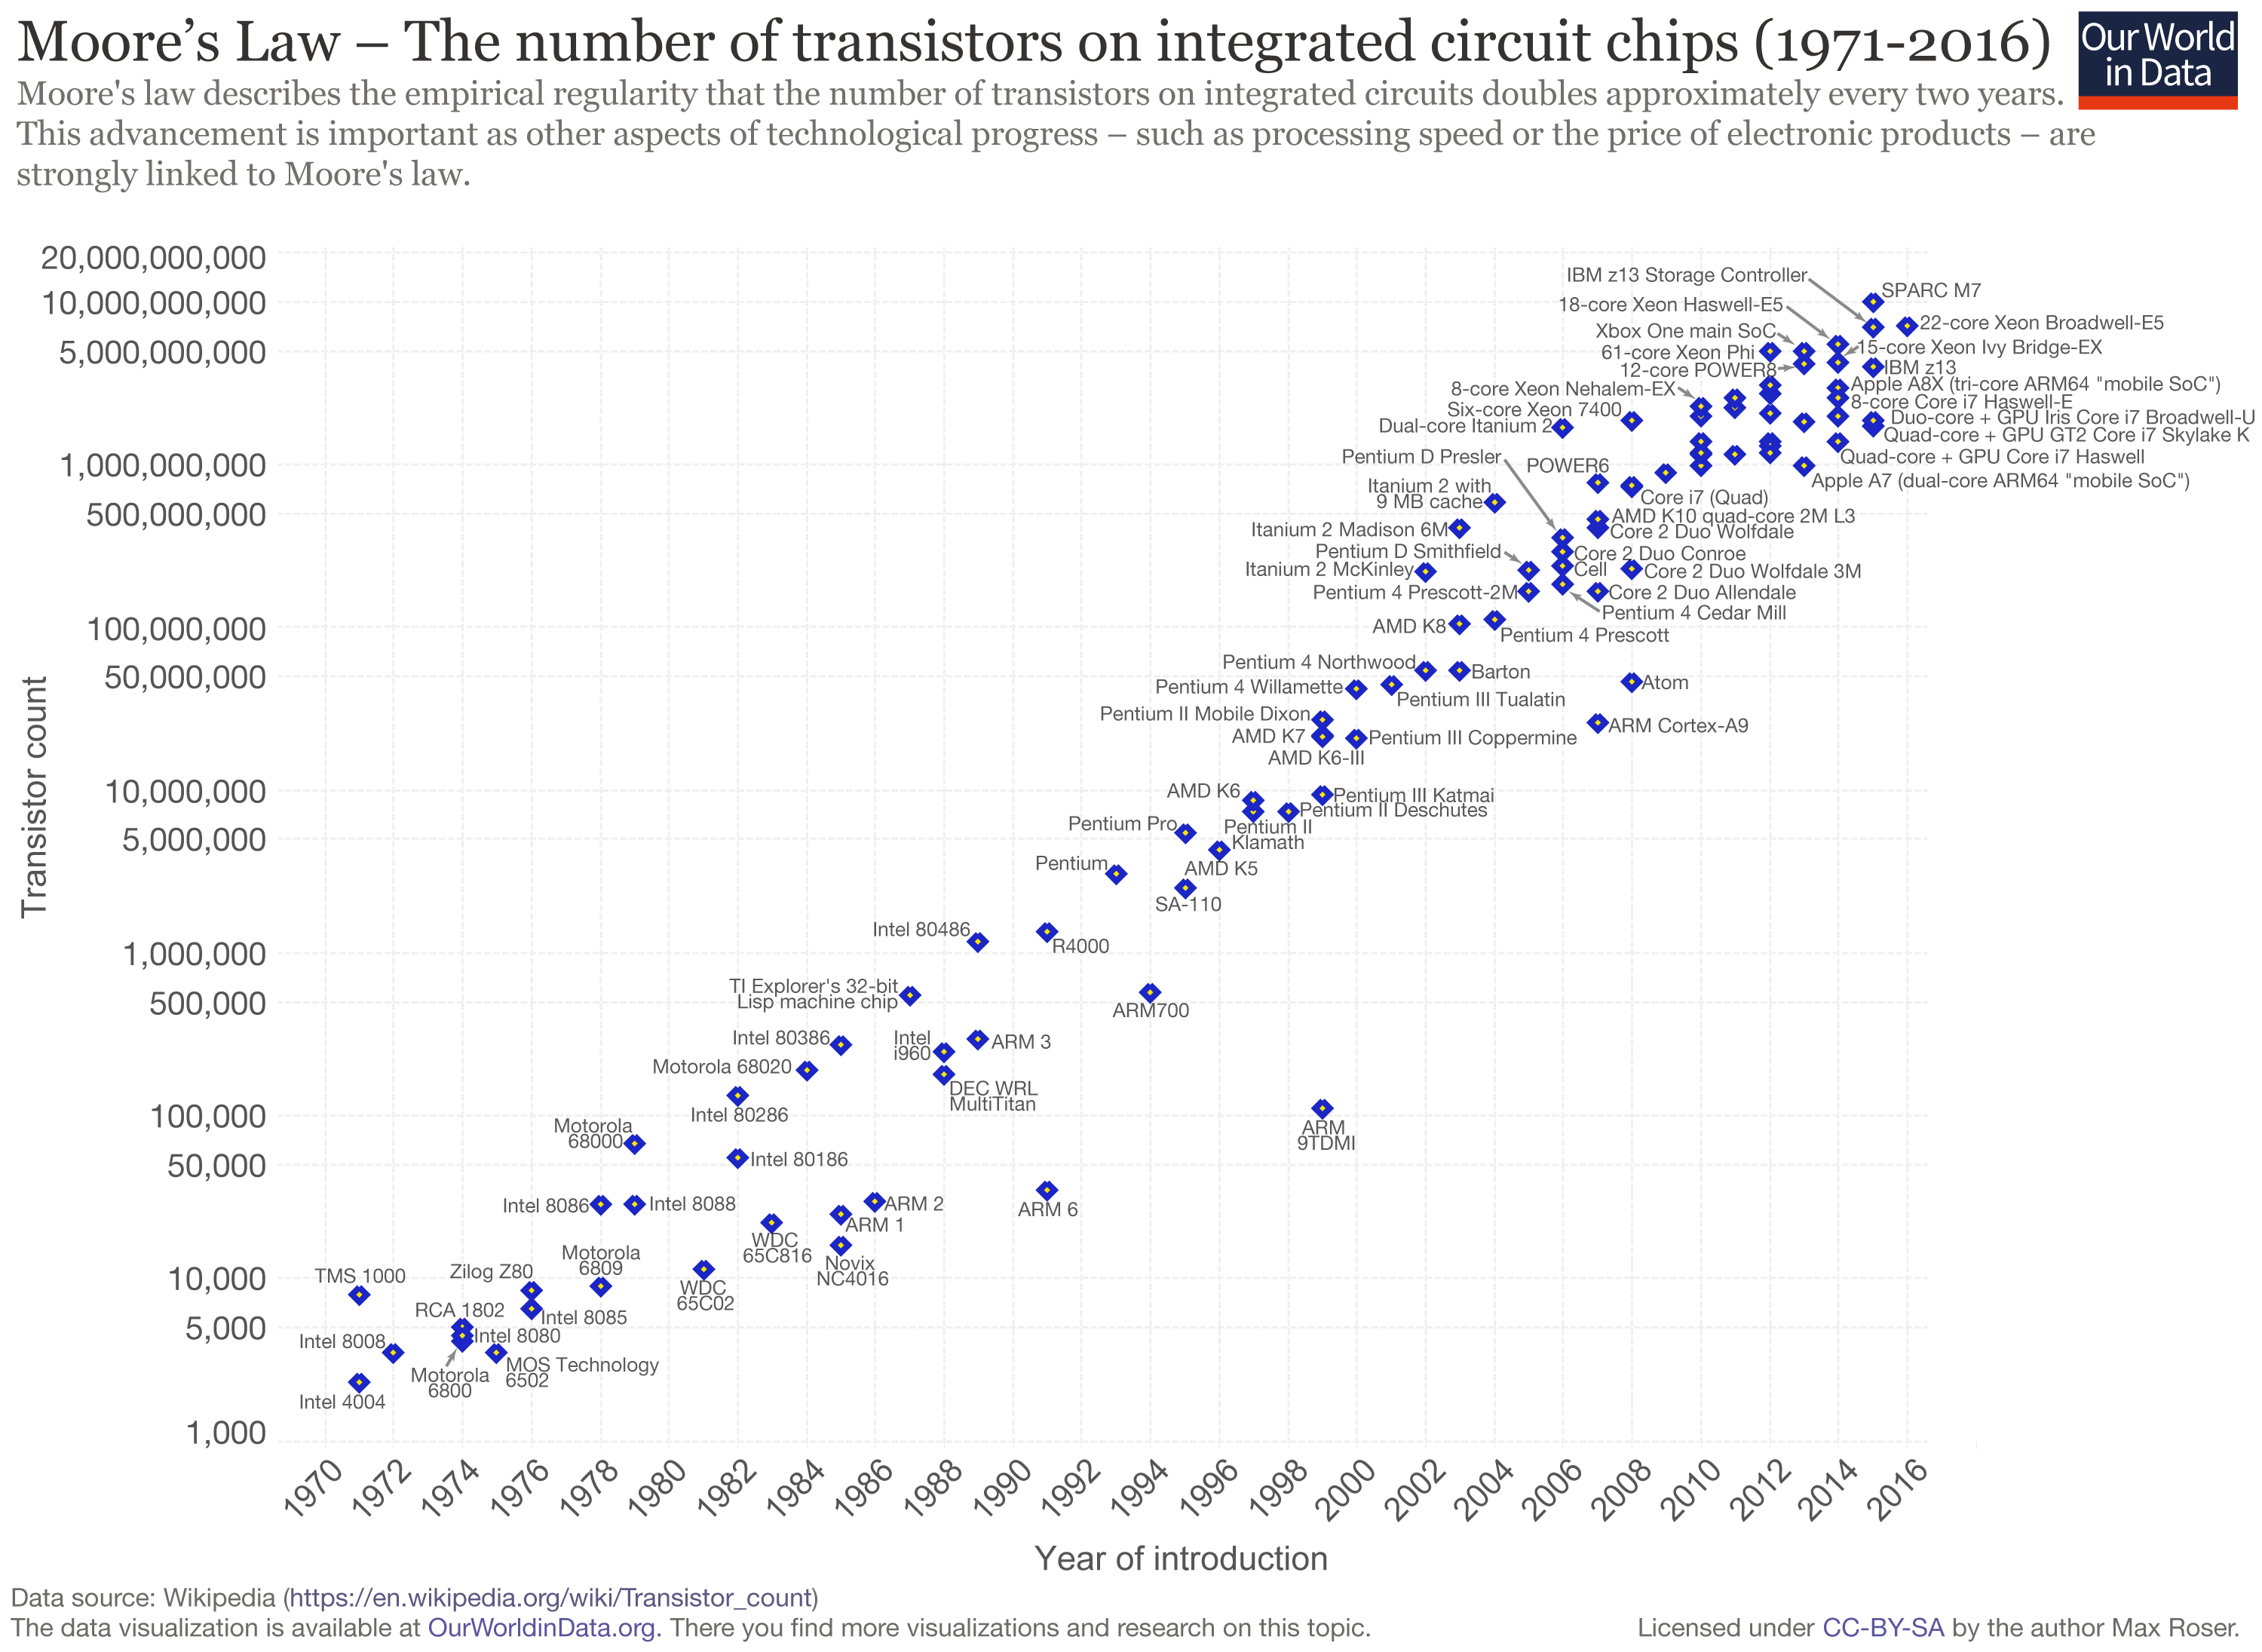
\includegraphics{moorelaw.png}
\caption{A graph that shows the number of transistors through the years.
We can see the glimpse of the recent decline}
\end{figure}

\subsection{The rise of Hardware}\label{the-rise-of-hardware}

Hardware and Software designate here respectively programs that are
executed as code for a general purpose processing unit and programs that
are encoded in the circuits. The dichotomy is not very well defined and
we can think of it as a spectrum. General-purpose computing on graphics
processing units (GPGPU) is in-between. Very efficient when appropriate
and used well. They have benefited from high-investment and many
generation of iterations and hence, for some tasks, can rivalize or even
surpass Hardware.

\begin{figure}
\centering
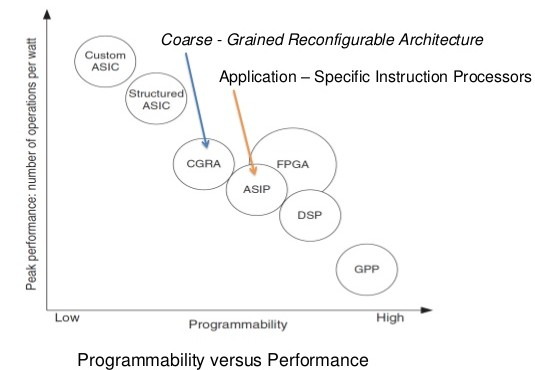
\includegraphics{hwsf.jpg}
\caption{Hardware vs Software}
\end{figure}

Hardware has always been there but application-specific integrated
circuit (ASIC) has prohibitive costs upfront (in the range of \$100M for
a tapeout). Reprogrammable hardware like field-programmable gate array
(FPGA) have only been used marginally and for some specific industry
like high-frequency trading. But now Hardware might be the only solution
(until a computing revolution happen, like quantum computing, but this
is not realist for the near future) to increase performance. But
hardware do not enjoy the same quality of tool, language and integrated
development environment (IDE) as software. This is the motivation behind
Spatial.

\subsection{Hardware as companion
accelerators}\label{hardware-as-companion-accelerators}

In most case, hardware would be inappropriate: running an OS as hardware
would be irrealist. However, as a companion to a central-processing unit
(CPU also called ``the host''), you are able to get the best of both
world. The flexibility of software on a CPU with the speed of hardware.
In this setup, hardware is considered an ``accelerator'' (Hence, the
term ``accelerating hardware''). It accelerates the most demanding
subroutines of the CPU. This companionship is already present in modern
computer desktops under the form of GPUs for \emph{shader} operations
and sound card for complex sound transformation/output.

\subsection{The right metric:
Perf/Watt}\label{the-right-metric-perfwatt}

The right metric for accelerator is performance by energy, as measured
in FLOPS per Watt. This is a fair metric for the comparison of different
hardware because it shows the intrisic value of the architecture. If the
metric was solely performance, then it would suffice to combine multiple
of the same architecture. Perf per dollar is not a good metric either
because you should also account for the cost of energy at runtime.
Hence, Perf/Watt seems like a fair metric to compare architectures.

\subsection{Spatial}\label{spatial}

At the dawn lab, under the lead of
\href{http://arsenalfc.stanford.edu/kunle}{Prof.~Kunle} and his grad
students, is developped a scala DSL
\href{https://github.com/stanford-ppl/spatial-lang}{spatial} and its
compiler to program Hardware in a higher-level, more user-friendly, more
productive language than Verilog. In particular, the control flows are
automatically generated when possible. This should enable software
engineers to unlock the potential of Hardware. A custom CGRA,
Plasticine, has been developped in parralel to Spatial. It leverages
some recurrent patterns, in particular parralel patterns and aims to be
the most efficient reprogrammable architecture for Spatial.

There is a large upfront cost but once at a big enough scale, Plasticine
could be deployed as an accelerator for most demanding server
applications and embedded systems with heavy computing requirements.

\subsection{Embedded systems and
drones}\label{embedded-systems-and-drones}

Embedded systems are limited by the amount of power at disposal from the
battery and might also have size constraints. At the same time,
especially for autonomous vehicles, there is a great need for computing
power.

Thus, developping drone applications with spatial demonstrates the
advantages of the platform. As a matter of fact, the filter that has
been developped was only made possible because it was run on an
accelerating hardware. It would be irrealist to attempt to run it on
more conventional micro-transistors. This is why the family in which
belong the filter developped here, particles filters, being very
computationally expensive, are very seldom used for drones.

\section{Part I: Accelerated optimal sensor fusion algorithm for POSE
estimation of drones: Asynchronous Rao-Blackwellized Particle
filter"}\label{part-i-accelerated-optimal-sensor-fusion-algorithm-for-pose-estimation-of-drones-asynchronous-rao-blackwellized-particle-filter}

Before expanding on the Rao-Blackwellized particle filter, we will
introduce here several other filters for POSE estimation for highly
dynamic objects: Complementary filter, Kalman Filter, Extended Kalman
Filter and finally Rao-Blackwellized Particle filter. The order is from
the most conceptually simple, to the most complex. This order is
justified not only for pedagogic purposes but also because
Rao-blackwellized particle filters use Kalman filters as one of their
building block.

\subsection{Drones and collision
avoidance}\label{drones-and-collision-avoidance}

The original motivation for the development of accelerated POSE
estimation is for the task of collision avoidance by quadcopters. In
particular, a collision avoidance algorithm developped at the
\href{https://asl.stanford.edu/}{ASL lab} and demonstrated here
\href{https://www.youtube.com/watch?v=kdlhfMiWVV0}{(https://youtu.be/kdlhfMiWVV0)}

\begin{figure}
\centering
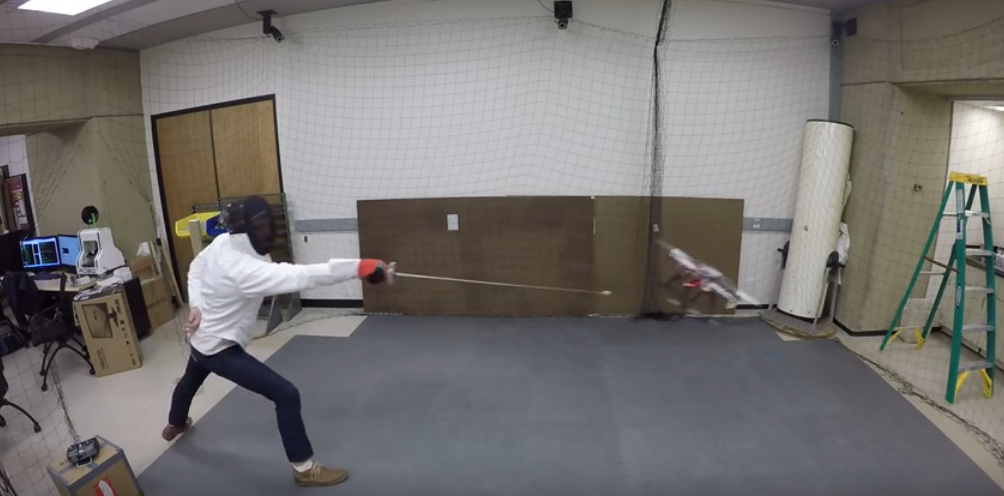
\includegraphics{fencing.png}
\caption{Ross Allen fencing with his drone}
\end{figure}

where the drone avoids the sword attack froms its creator. At first, it
was thought of accelerating the whole algorithm but it was found that
one of the most demanding subroutine was pose estimation. POSE is the
combination of the position and orientation of an object. Moreover, it
was wished to increase the processing rate of the filter such that it
could match the input with the fastest sampling rate: its inertial
measurement unit (IMU) containing an accelerometer, a gyroscope and a
magnetometer.

The flamewheel f450 is the typical drone in this category. It is
surprisingly fast and agile. Given the proper command, it can generate
enough thrust to avoid in a very short lapse of time any incoming
object.

\begin{figure}
\centering
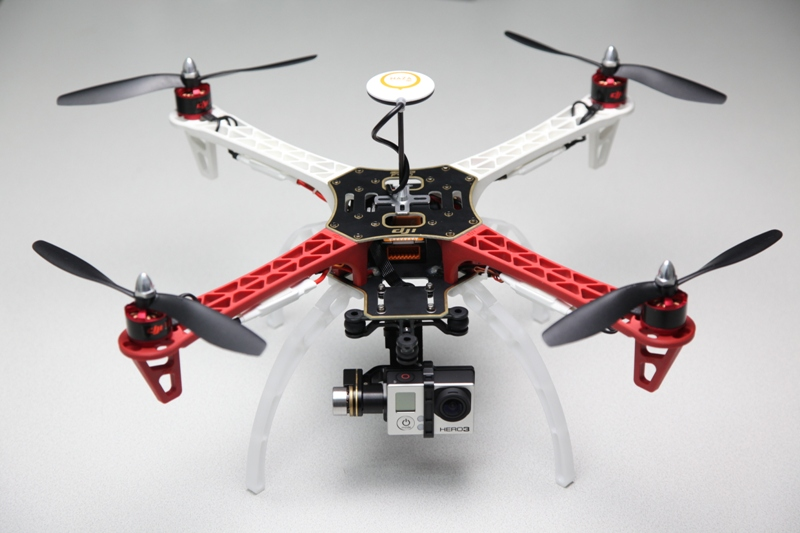
\includegraphics{f450.jpg}
\caption{The Flamewheel f450}
\end{figure}

\subsection{Sensor fusion}\label{sensor-fusion}

Sensor fusion is combining of sensory data or data derived from
disparate sources such that the resulting information has less
uncertainty than would be possible when these sources were used
individually. In the context of drones, it is very useful because it
enables to combine many unprecise sensor measurement to form a more
precise measurement like having precise positionning from 2 less precise
GPS (dual GPS setting). It can also permit to combine sensors with
different sampling rates: typically precise sensors with low sampling
rate and less precise sensors with high sampling rate. Both cases are
gonna be relevant here.

A fundamental explanation why this is possible comes from the central
limit theorem: one sample from a distribution with a low variance is as
good as n sample from a distribution with variance \(n\) times higher.

\[\mathbb{V}(X_i)=\sigma^2 ~~~~~ \mathbb{E}(X_i) = \mu\]
\[\bar{X} = \frac{1}{n}\sum X_i\]
\[\mathbb{V}(\bar{X}) = \frac{\sigma^2}{n}  ~~~~~ \mathbb{E}(\bar{X}) = \mu\]

\subsection{Notes on notation and
conventions}\label{notes-on-notation-and-conventions}

The referential by default is the fixed world frame.

\begin{itemize}
\tightlist
\item
  \(\mathbf{x}\) designates a vector
\item
  \(x_t\) is the random variable of x at time t
\item
  \(x_{t1:t2}\) is the product of the random variable of x between t1
  included and t2 included
\item
  \(x^{(i)}\) designates the random variable x of the arbitrary particle
  i
\item
  \(\hat{x}\) designates an estimated variable
\end{itemize}

\subsection{POSE}\label{pose}

POSE is the task of estimating the position and orientation of an object
through time. It is a subroutine of Software Localization And Mapping
(SLAM). We can formelize the problem as:

At each timestep, find the best expectation of a function of the hidden
variable state (position and orientation), from their initial
distribution and the history of observable random variables (such as
sensor measurements).

\begin{itemize}
\tightlist
\item
  The state \(\mathbf{x}\)
\item
  The function \(g(\mathbf{x})\) such that
  \(g(\mathbf{x}_t) = (\mathbf{p}_t, \mathbf{q}_t)\) where
  \(\mathbf{p}\) is the position and \(\mathbf{q}\) is the attitude as a
  quaternion.
\item
  The observable variable \(\mathbf{y}\) composed of the sensor
  measurements \(\mathbf{z}\) and the control input \(\mathbf{u}\)
\end{itemize}

The algorithm inputs are:

\begin{itemize}
\tightlist
\item
  control inputs \(\mathbf{u}_t\) (the commands sent to the flight
  controller)
\item
  sensor measurements \(\mathbf{z}_t\) coming from different sensors
  with different sampling rate
\item
  information about the sensors (sensor measurements biases and matrix
  of covariance)
\end{itemize}

\subsection{Quaternion}\label{quaternion}

Quaternions are extensions of complex numbers but with 3 imaginary
parts. Unit quaternions can be used to represent orientation, also
referred to as attitude. Quaternions algebra make rotation composition
simple and quaternions avoid the issue of gimbal lock. In all filters
presented, they will be used to represent the attitude.

Quaternion rotations composition is: \(q_2 q_1\) which results in
\(q_1\) being rotated by the rotation represented by \(q_2\). From this,
we can deduce that angular velocity integrated over time is simply
\(q^t\) if \(q\) is the local quaternion rotation by unit of time.

Rotation of a vector by a quaternion is done by: \(q v q^*\) where \(q\)
is the quaternion representing the rotation, \(q^*\) its conjugate and
\(v\) the vector to be rotated.

\subsection{Helper functions and
matrices}\label{helper-functions-and-matrices}

We introduce some helper matrices.

\begin{itemize}
\tightlist
\item
  \(\mathbf{R}_{b2f}\{\mathbf{q}\}\) is the body to fixed vector
  rotation matrix. It transforms vector in the body frame to the fixed
  world frame. It takes as parameter the attitude \(\mathbf{q}\).
\item
  \(\mathbf{R}_{f2b}\{\mathbf{q}\}\) is its inverse matrix (from fixed
  to body).
\item
  \(\mathbf{T}_{2a} = (0, 0, 1/m)^T\) is the scaling from thrust to
  acceleration (by dividing by the weight of the drone:
  \(\mathbf{F} = m\mathbf{a} \Rightarrow \mathbf{a} = \mathbf{F}/m)\)
  and then multiplying by a unit vector \((0, 0, 1)\)
\item
  \[R2Q(\boldsymbol{\theta}) = (\cos(\| \boldsymbol{\theta} \| / 2), \sin(\| \boldsymbol{\theta} \| / 2) \frac{\boldsymbol{\theta}}{\| \boldsymbol{\theta} \|} )\]
  is a function that convert from a local angle rotation to a local
  quaternion rotation. The definition of this function come from
  converting \(\boldsymbol{\theta}\) to a body-axis angle, and then to a
  quaternion.
\item
  \[Q2R(\mathbf{q}) = (q.i*s, q.j*s, q.k*s) \] is its inverse function
  where \(n = \arccos(q.w)*2\) and \(s = n/\sin(n/2)\)
\item
  \(\Delta t\) is the lapse of time between t and the next tick (t+1)
\end{itemize}

\subsection{Model}\label{model}

The drone is assumed to have rigid-body physics. It is submitted to the
gravity and its own inertia. A rigid body is a solid body in which
deformation is zero or so small it can be neglected. The distance
between any two given points on a rigid body remains constant in time
regardless of external forces exerted on it. This enable to summarise
the forces from the rotor as a thrust oriented in the direction normal
to the plane formed by the 4 rotosrs, and an angular velocity.

Those variables are sufficient to describe the evolution of our drone
with rigid-body physics:

\begin{itemize}
\tightlist
\item
  \(\mathbf{a}\) the total acceleration in the fixed world frame
\item
  \(\mathbf{v}\) the velocity in the fixed world frame
\item
  \(\mathbf{p}\) the position in the fixed world frame
\item
  \(\boldsymbol{\omega}\) the angular velocity
\item
  \(\mathbf{q}\) the attitude in the fixed world frame
\end{itemize}

\subsection{Sensors}\label{sensors}

The sensors at disposition are:

\begin{itemize}
\item
  \textbf{Accelerometer}: It generates \(\mathbf{a_A}\) a measurement of
  the total acceleration in the body frame referrential the drone is
  submitted to at a \textbf{high} sampling rate. If the object is
  submitted to no acceleration then the accelerometer measure the
  earth's gravity field from. From that information, it could be
  possible to retrieve the attitude. Unfortunately, we are in a highly
  dynamic setting. Thus, it is possible when we can substract the
  drone's acceleration from the thrust to the total acceleration. This
  would require to know exactly the force exerced by the rotors at each
  instant. In this work, we assume that doing that separation, while
  being theoretically possible, is too impractical. The measurements
  model is:
  \[\mathbf{a_A}(t) = \mathbf{R}_{f2b}\{\mathbf{q}(t)\}\mathbf{a}(t) + \mathbf{a_A}^\epsilon\]
  where the covariance matrix of the noise of the accelerometer is
  \({\mathbf{R}_{\mathbf{a_A}}}_{3 \times 3}\) and
  \[\mathbf{a_A}^\epsilon \sim \mathcal{N}(\mathbf{0}, \mathbf{R}_{\mathbf{a_A}})\].
\item
  \textbf{Gyroscope}:It generates \(\mathbf{\boldsymbol{\omega}_G}\) a
  measurement of the angular velocity in the body frame of the drone at
  the last timestep at a \textbf{high} sampling rate. The measurement
  model is:
  \[\mathbf{\boldsymbol{\omega}_G}(t) = \boldsymbol{\omega} + \mathbf{\boldsymbol{\omega}_G}^\epsilon\]
  where the covariance matrix of the noise of the accelerometer is
  \({\mathbf{R}_{\mathbf{\boldsymbol{\omega}_G}}}_{3 \times 3}\) and
  \[\mathbf{\boldsymbol{\omega}_G}^\epsilon_t \sim \mathcal{N}(\mathbf{0}, \mathbf{R}_{\mathbf{\boldsymbol{\omega}_G}})\].
\item
  \textbf{Position}: It generates \(\mathbf{p_V}\) a measurement of the
  current positionat a \textbf{low} sampling rate. This is usually
  provided by a \textbf{Vicon} (for indoor), \textbf{GPS}, a
  \textbf{Tango} or any other position sensor. The measurement model is:
  \[\mathbf{p_V}(t) = \mathbf{p}(t) + \mathbf{p_V}^\epsilon\] where the
  covariance matrix of the noise of the position is
  \({\mathbf{R}_{\mathbf{p_V}}}_{3 \times 3}\) and
  \[\mathbf{p_V}^\epsilon \sim \mathcal{N}(\mathbf{0}, \mathbf{R}_{\mathbf{p_V}})\].
\item
  \textbf{Attitude}: It generates \(\mathbf{q_V}\) a measurement of the
  current attitute. This is usually provided in addition to the position
  by a \textbf{Vicon} or a \textbf{Tango} at a \textbf{low} sampling
  rate or the \textbf{Magnemoter} at a \textbf{high} sampling rate if
  the environment permit it (no high magnetic interference nearby like
  iron contamination). The magnetometer retrieve the attitude by
  assuming that the sensed magnetic field corresponds to the earth's
  magnetic field. The measurement model is:
  \[\mathbf{q_V}(t) = \mathbf{q}(t)*R2Q(\mathbf{q_V}^\epsilon)\] where
  the \(3 \times 3\) covariance matrix of the noise of the attitude in
  radian before being converted by \(R2Q\) is
  \({\mathbf{R}_{\mathbf{q_V}}}_{3 \times 3}\) and
  \[\mathbf{q_V}^\epsilon \sim \mathcal{N}(\mathbf{0}, \mathbf{R}_{\mathbf{q_V}})\].
\item
  \textbf{Optical Flow}: A camera that keeps track of the movement by
  comparing the difference of the position of some reference points. By
  using a companion distance sensor, it is able to retrieve the
  difference between the two perspective and thus the change in angle
  and position.
  \[\mathbf{dq_O}(t) = (\mathbf{q}(t-k)\mathbf{q}(t))*R2Q(\mathbf{dq_O}^\epsilon)\]
  \[\mathbf{dp_O}(t) = (\mathbf{p}(t) - \mathbf{p}(t-k)) + \mathbf{dp_O}^\epsilon\]
\end{itemize}

where the \(3 \times 3\) covariance matrix of the noise of the attitude
variation in radian before being converted by \(R2Q\) is
\({\mathbf{R}_{\mathbf{dq_O}}}_{3 \times 3}\) and
\[\mathbf{dq_O}^\epsilon \sim \mathcal{N}(\mathbf{0}, \mathbf{R}_{\mathbf{dq_O}})\]
and the position variation covariance matrix
\({\mathbf{R}_{\mathbf{dp_O}}}_{3 \times 3}\) and
\[\mathbf{dp_O}^\epsilon \sim \mathcal{N}(\mathbf{0}, \mathbf{R}_{\mathbf{dp_O}})\].

\begin{figure}
\centering
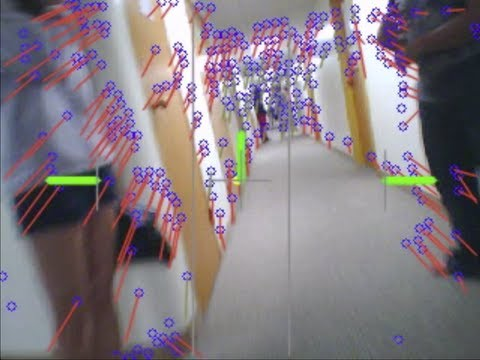
\includegraphics{opflow.jpg}
\caption{Optical flow from a moving drone}
\end{figure}

The notable difference with the position or attitude sensor is that the
optical flow sensor, like the IMU, only captures time variation, not
absolute values.

\begin{itemize}
\tightlist
\item
  \textbf{Altimeter}: An altimeter is a sensor that measure the altitude
  of the drone. For instance a LIDAR measure the time for the laser wave
  to reflect on a surface that is assumed to be the ground. A smart
  strategy is to only use the altimeter is oriented with a low angle to
  the earth, else you also have to account that angle in the estimation
  of the altitude.
  \[z_A(t) = \sin(\text{pitch}(\mathbf{q(t)}))(\mathbf{p}(t).z + z_A^\epsilon)\]
  \({R_{z_A}}_{3 \times 3}\) and
  \[z_A^\epsilon \sim \mathcal{N}(0, R_{z_A})\]
\end{itemize}

\begin{figure}
\centering
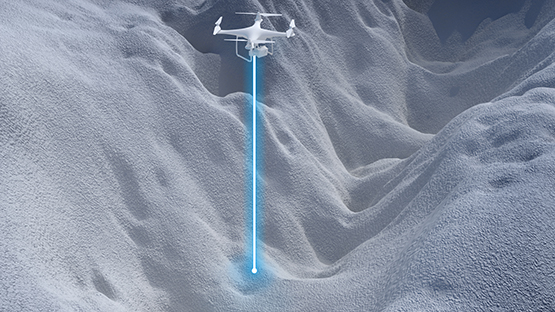
\includegraphics{altimeter.jpg}
\caption{Rendering of the LIDAR laser of an altimeter}
\end{figure}

Some sensors are more relevant indoor and some others outdoor:

\begin{itemize}
\tightlist
\item
  \textbf{Indoor}: The sensors available indoor are the accelerometer,
  the gyroscope and the \textbf{Vicon}. The Vicon is a system composed
  of many sensors around a room that is able to track very accurately
  the position and orientation a mobile object. One issue with relying
  solely on the \textbf{Vicon} is that the sampling rate is low.
\end{itemize}

\begin{figure}
\centering
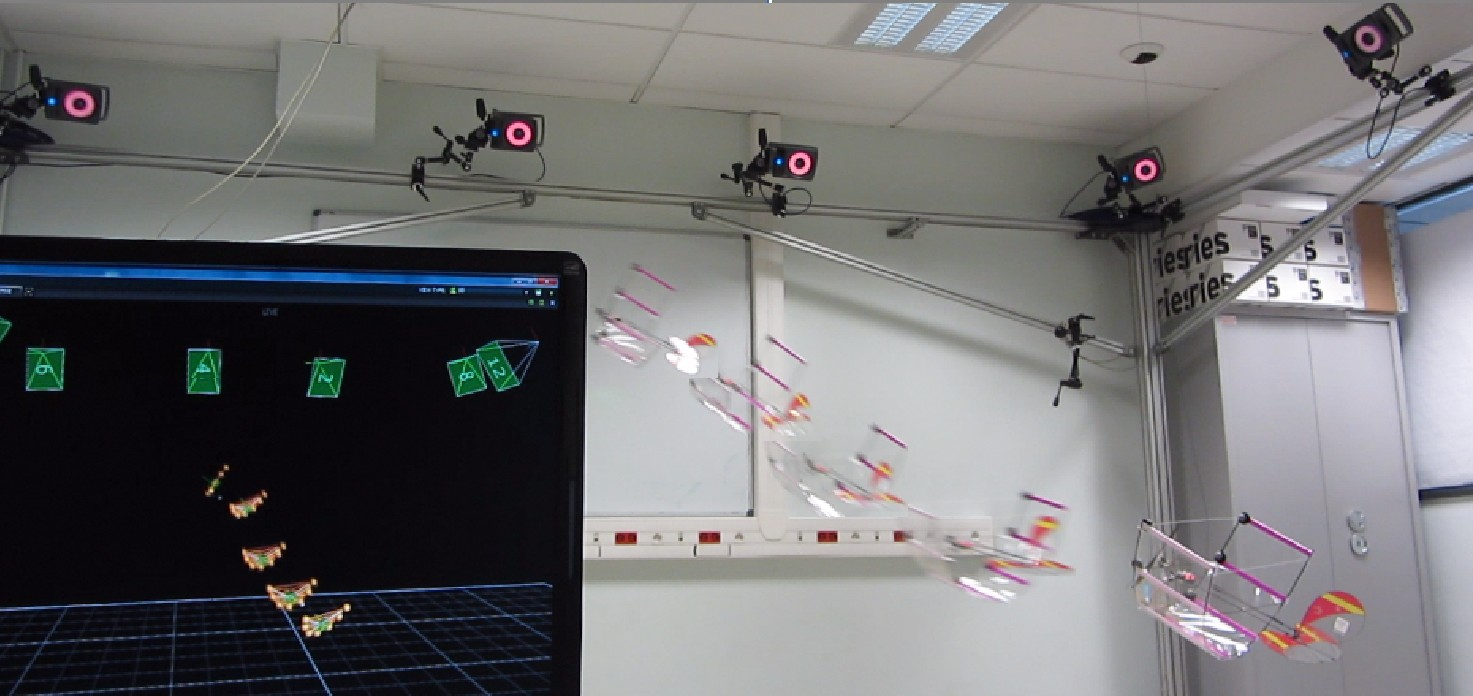
\includegraphics{vicon.jpg}
\caption{A Vicon setup}
\end{figure}

\begin{itemize}
\tightlist
\item
  \textbf{Outdoor}: The sensors available outdoor are the accelerometer,
  the gyroscope, the magnetometer, two GPS, an optical flow and an
  altimeter.
\end{itemize}

We assume that since the biases of the sensor could be known prior to
the flight, the sensor have been calibrated and output measurements with
no bias. Some filters like the
\href{https://dev.px4.io/en/tutorials/tuning_the_ecl_ekf.html}{ekf2} of
the px4 flight stack keep track of the sensor biases but this is a state
augmentation that was not deemed worthwhile.

\subsubsection{Control inputs}\label{control-inputs}

Observations from the control input are not strictly speaking
measurements but input of the state-transition model. The IMU is a
sensor, thus stricly speaking, its measurements are not control inputs.
However, in the literature, it is standard to use its measurements as
control inputs. One of the advantage is that the accelerometer measures
acceleration and angular velocity, raw values close from the input we
need in our state-transition. If we used a transformation of the thrust
sent as command to the rotors, we would have to account for the rotors
unprecision, the wind and other disturbances. Another advantage is that
since the IMU has very high sampling rate, we can update very frequently
the state with new transitions. The drawback is that the accelerometer
is noisy. Fortunately, we can take into account the noise as a process
model noise.

The control inputs at disposition are:

\begin{itemize}
\tightlist
\item
  \textbf{Acceleration}: \(\mathbf{a_A}_t\) from the acceloremeter
\item
  \textbf{Angular velocity}: \(\mathbf{\boldsymbol{\omega}_G}_t\) from
  the gyroscope.
\end{itemize}

\hypertarget{model-dynamic}{\subsubsection{Model
dynamic}\label{model-dynamic}}

\begin{itemize}
\tightlist
\item
  \(\mathbf{a}(t+1) = \mathbf{a_A}_t + \mathbf{a_A}^\epsilon_t\) where
  \(\mathbf{a}^\epsilon_t \sim \mathcal{N}(\mathbf{0}, \mathbf{Q}_{\mathbf{a}_t })\)
\item
  \(\mathbf{v}(t+1) = \mathbf{v}(t) + \Delta t \mathbf{a}(t) + \mathbf{v}^\epsilon_t\)
  where
  \(\mathbf{v}^\epsilon_t \sim \mathcal{N}(\mathbf{0}, \mathbf{Q}_{\mathbf{v}_t })\)
\item
  \(\mathbf{p}(t+1) = \mathbf{p}(t) + \Delta t \mathbf{v}(t) + \mathbf{p}^\epsilon_t\)
  where
  \(\mathbf{p}^\epsilon_t \sim \mathcal{N}(\mathbf{0}, \mathbf{Q}_{\mathbf{p}_t })\)
\item
  \(\boldsymbol{\omega}(t+1) = \mathbf{\boldsymbol{\omega}_G}_t + \mathbf{\boldsymbol{\omega}_G}^\epsilon_t\)
  where
  \(\mathbf{p}^\epsilon_t \sim \mathcal{N}(\mathbf{0}, \mathbf{Q}_{\mathbf{\boldsymbol{\omega}_G}_t })\)
\item
  \(\mathbf{q}(t+1) = \mathbf{q}(t)*R2Q(\Delta t \boldsymbol{ \omega(t) })\)
\end{itemize}

Note that in our model, \(\mathbf{q}(t+1)\) must be known. Fortunately,
as we will see later, our RBPF is conditionned under the attitude so it
is known.

\subsection{State}\label{state}

The time series of the variables of our dynamic model constitute a
hidden markov chain. Indeed, the model is ``memoryless'' and depend only
on the current state and of a sampled transition.

States contain variables that enable us to keep track of some of those
hidden variables which is our ultimate goal (for POSE \(\mathbf{p}\) and
\(\mathbf{q}\)). States at time \(t\) are denoted by \(\mathbf{x}_t\).
Different filters require different state variables depending on their
structure and assumptions.

\subsection{Observation}\label{observation}

Observations are revealed variables conditionned under the variables of
our dynamic model. Our ultimate goal is to deduce the states from the
observations.

Observations contain the control input \(\mathbf{u}\) and the
measurements \(\mathbf{z}\).

\[\mathbf{y}_t = (\mathbf{z}_t, \mathbf{u}_t)^T = (\mathbf{p_V}_t, \mathbf{q_V}_t), ({t_C}_t, \mathbf{\boldsymbol{\omega}_C}_t))^T\]

\subsection{Filtering and smoothing}\label{filtering-and-smoothing}

\textbf{Smoothing} is the statistical task of finding the expectation of
the state variable from the past history of observations and multiple
observation variables ahead

\[\mathbb{E}[g(\mathbf{x}_{0:t}) | \mathbf{y}_{1:t+k}]\]

Which expand to,

\[\mathbb{E}[(\mathbf{p}_{0:t}, \mathbf{q}_{0:t}) | (\mathbf{z}_{1:t+k}, \mathbf{u}_{1:t+k})]\]

\(k\) is a contant and the first observation is \(y_1\)

\textbf{Filtering} is a kind of smoothing where you only have at
disposal the current observation variable (\(k=0\))

\section{Complementary Filter}\label{complementary-filter}

The complementary filter is the simplest of all and very common to
retrieve the attitude on low-computing systems because of its low
computational complexity. The gyroscope and accelerometer both provide a
measurement that can help us to estimate the attitude. The gyroscope
indeed gives us a noisy measurement of the angular velocity from which
we can retrieve the new attitude from the past one by time integration:
\(\mathbf{q}_t = \mathbf{q}_{t-1}*R2Q(\Delta t \mathbf{\omega})\). This
is commonly called ``Dead reckoning''\footnote{The etymology for ``Dead
  reckoning'' comes from the mariners of the XVIIth century that used to
  calculate the position of the vessel with log book. The interpretation
  of ``dead'' is subject to debate. Some argue that it is a mispelling
  of ``ded'' as in ``deduced''. Others argue that it should be read by
  its old meaning: \emph{absolute}.} and is prone to accumulation error,
referred as drift. Indeed, like brownian motions, even if the process is
unbiased, the variance grows with time. Reducing the noise cannot solve
the issue entirely: even with extremely precise instruments, you are
subject to floating point errors.

Fortunately, the accelerometer gives us a highly unprecise measurement
of the orientation but is not subject to drift. Indeed, if not subject
to other accelerations, the accelerometer measures the gravity field
orientation. Since this field is oriented toward earth, it is possible
to retrieve the current rotation from that field and by extension the
attitude. However, in the case of a drone, it is subject to continuous
and signifiant acceleration and vibration. Hence, the assumption that we
retrieve the gravity field directly is wrong. We can solve this by
substracting the acceleration deduced from the thrust control input.

\textbf{TODO} pictures

The idea of the filter is to combine the precise short-term measurements
of the gyroscope subject to drift with the ``long-term'' measurements of
the accelerometer.

\textbf{TODO}: continue

\section{Augmented Complementary
Filter}\label{augmented-complementary-filter}

\section{Kalman Filter}\label{kalman-filter}

\subsection{Linearity}\label{linearity}

Kalman filters are optimal linear filters. Hence, Kalman filters are non
optimal for our problem because our state has some non-linear components
(attitude).Indeed, rotations and attitudes belong to \(SO(3)\) which is
not a vector space. Therefore, we cannot use vanilla kalman filters.
However, understanding kalman filters give us a good understanding of
Bayesian inference and the filters that we will present after use Kalman
filters or are extensions of them to deal with non-linearity. One
example of such extension is the extended kalman filter that we will
present in the following section.

\textbf{TODO}: Kalman explanataion

\subsection{Extended Kalman Filters}\label{extended-kalman-filters}

EKF are linearized Kalman filters of the first order.

An EKF is semi-developped in the annex.

\textbf{TODO}: EKF explanations

\subsection{Unscented Kalman Filters}\label{unscented-kalman-filters}

\textbf{TODO}: UKF explanations

\section{Particle Filter}\label{particle-filter}

Particle filters are computionally expensive and that is why their usage
is not very popular currently for low-powered embedded systems.

Particle filters are monte carlo methods which in their general form
\ldots{} \textbf{TODO}

\textbf{TODO}

\subsection{Average quaternion}\label{average-quaternion}

Unfortunately, the average of quaternions components
\(\frac{1}{N} \sum q_i\) or \emph{barycentric} mean is unsound: Indeed,
attitude do not belong to a vector space but a homogenous Riemannian
manifold (the four dimensional unit sphere). To convince yourself of the
unsoundness of the \emph{barycentric} mean, see that the addition and
barycentric mean of two unit quaternion is not necessarily an unit
quaternion (\((1, 0, 0, 0)\) and \((-1, 0, 0, 0)\) for instance.
Furthermore, angle being periodic, the \emph{barycentric} mean of a
quaternion with angle \(-178^\circ\) and another with same body-axis and
angle \(180^\circ\) gives \(1^\circ\) instead of the expected
\(-179^\circ\).

To calculate the average quaternion, we use an algorithm which minimize
a metric that correspond to the weighted attitude difference to the
average, namely the weighted sum of the squared Frobenius norms of
attitude matrix differences.
\[\bar{\mathbf{q}} = arg \min_{q \in \mathbb{S}^3} \sum w_i \| A(\mathbf{q}) - A(\mathbf{q}_i) \|^2_F\]

where \(\mathbb{S}^3\) denotes the unit sphere.

The attitude matrix \(A(\mathbf{q})\) and its corresponding Frobenius
norm are out of scope of this work but can be found in more details in
(Markley et al. \protect\hyperlink{ref-markley_averaging_2007}{2007})

\subsection{Resampling}\label{resampling}

When the number of effective particles is too low (\(N/10\)), we apply
systematic resampling

\section{Rao-Blackwellized Particle
Filter}\label{rao-blackwellized-particle-filter}

\subsection{Introduction}\label{introduction-1}

Compared to a plain PF, RPBF leverage the linearity of some components
of the state by assuming our model gaussian conditionned on a latent
variable: Given the attitude \(q_t\), our model is linear. This is where
RPBF shines: We use particle filtering to estimate our latent variable,
the attitude, and we use the optimal kalman filter to estimate the state
variable.

This main inspiration from this approach is (Vernaza and Lee
\protect\hyperlink{ref-vernaza_rao-blackwellized_2006}{2006}). However,
it differs by:

\begin{itemize}
\tightlist
\item
  adapt the filter to drones by taking into account that the system is
  too dynamic for assuming that the accelerometer simply output the
  gravity vector. This is solved by augmenting the state with the
  acceleration as shown later.
\item
  not use measurements of the IMU as control inputs (this is usually
  used for wheeled vehicles because of the drift from the wheels) but
  have both control inputs and measurements.
\item
  add an attitude sensor.
\end{itemize}

We introduce the latent variable \(\boldsymbol{\theta}\)

The latent variable \(\boldsymbol{\theta}\) has for sole component the
attitude: \[\boldsymbol{\theta} = (\mathbf{q})\]

\(q_t\) is estimated from the product of the attitude of all particles
\(\mathbf{\theta^{(i)}} = \mathbf{q}^{(i)}_t\) as the ``average''
quaternion \(\mathbf{q}_t = avgQuat(\mathbf{q}^n_t)\). \(x^n\)
designates the product of all n arbitrary particle.

We use importance sampling \ldots{} \textbf{TODO}

The weight definition is:

\[w^{(i)}_t = \frac{p(\boldsymbol{\theta}^{(i)}_{0:t} | \mathbf{y}_{1:t})}{\pi(\boldsymbol{\theta}^{(i)}_{0:t} | \mathbf{y}_{1:t})}\]

From the definition, it is proovable that:

\[w^{(i)}_t \propto \frac{p(\mathbf{y}_t | \boldsymbol{\theta}^{(i)}_{0:t-1}, \mathbf{y}_{1:t-1})p(\boldsymbol{\theta}^{(i)}_t | \boldsymbol{\theta}^{(i)}_{t-1})}{\pi(\boldsymbol{\theta}^{(i)}_t | \boldsymbol{\theta}^{(i)}_{1:t-1}, \mathbf{y}_{1:t})} w^{(i)}_{t-1}\]

We choose the dynamic of the model as the importance distribution:

\[\pi(\boldsymbol{\theta}^{(i)}_t | \boldsymbol{\theta}^{(i)}_{1:t-1}, \mathbf{y}_{1:t}) = p(\boldsymbol{\theta}^{(i)}_t | \boldsymbol{\theta}^{(i)}_{t-1}) \]

Hence,

\[w^{(i)}_t \propto p(\mathbf{y}_t | \boldsymbol{\theta}^{(i)}_{0:t-1}, \mathbf{y}_{1:t-1}) w^{(i)}_{t-1}\]

We then sum all \(w^{(i)}_t\) to find the normalization constant and
retrieve the actual \(w^{(i)}_t\)

\subsection{State}\label{state-1}

\[\mathbf{x}_t = (\mathbf{w}_t, \mathbf{a}_t, \mathbf{v}_t, \mathbf{p}_t)^T\]

Initial state \(\mathbf{x}_0 = (\mathbf{0}, \mathbf{0}, \mathbf{0})\)

Initial covariance matrix
\(\mathbf{\Sigma}_{9 \times 9} = \epsilon \mathbf{I}_{9 \times 9}\)

\subsection{Latent variable}\label{latent-variable}

\[\mathbf{q}^{(i)}_{t+1} = \mathbf{q}^{(i)}_t*R2Q({\Delta t} (\mathbf{\boldsymbol{\omega}_C}_t+\mathbf{\boldsymbol{\omega}_C}^\epsilon_t))\]

\(\mathbf{\boldsymbol{\omega}_C}^\epsilon_t\) represents the error from
the control input and is sampled from
\(\mathbf{\boldsymbol{\omega}_C}^\epsilon_t \sim \mathcal{N}(\mathbf{0}, \mathbf{R}_{\mathbf{\boldsymbol{\omega}_C}_t })\)

Initial attitude \(\mathbf{q_0}\) is sampled such that the drone pitch
and roll are none (parralel to the ground) but the yaw is unknown and
uniformly distributed.

Note that \(\mathbf{q}(t+1)\) is known in the
\protect\hyperlink{model-dynamic}{model dynamic} because the model is
conditionned under \(\boldsymbol{\theta}^{(i)}_{t+1}\).

\subsection{Measurement model}\label{measurement-model}

\begin{enumerate}
\def\labelenumi{\arabic{enumi}.}
\tightlist
\item
  Accelerometer:
  \[\mathbf{a_A}(t) = \mathbf{R}_{f2b}\{\mathbf{q}(t)\}\mathbf{a}(t) + \mathbf{a_A}^\epsilon_t\]
  where
  \(\mathbf{a_A}^\epsilon_t \sim \mathcal{N}(\mathbf{0}, \mathbf{R}_{\mathbf{a_A}_t })\)
\item
  Gyroscope:
  \[\mathbf{\boldsymbol{\omega}_G}(t) = Q2R({\mathbf{q}^{(i)}(t-1)}^{-1}\mathbf{q}^{(i)}(t))/\Delta t + \mathbf{\boldsymbol{\omega}_G}^\epsilon(t)\]
  where
  \(\mathbf{\boldsymbol{\omega}_G}^\epsilon_t \sim \mathcal{N}(\mathbf{0}, \mathbf{R}_{\mathbf{\boldsymbol{\omega}_G}})\)
\item
  Position:
  \[\mathbf{p_V}(t) = \mathbf{p}(t)^{(i)} + \mathbf{p_V}^\epsilon_t\]
  where
  \(\mathbf{p_V}^\epsilon_t \sim \mathcal{N}(\mathbf{0}, \mathbf{R}_{\mathbf{p_V}_t })\)
\item
  Attitude:
  \[\mathbf{q_V}(t) = \mathbf{q}(t)^{(i)}*R2Q(\mathbf{q_V}^\epsilon_t)\]
  where
  \(\mathbf{q_V}^\epsilon_t \sim \mathcal{N}(\mathbf{0}, \mathbf{R}_{\mathbf{q_V}_t })\)
\end{enumerate}

\subsection{Kalman prediction}\label{kalman-prediction}

The model dynamics define the following model, state-transition matrix
\(\mathbf{F}_t\{\boldsymbol{\theta}^{(i)}_t\}\), the control-input
matrix \(\mathbf{B}_t\{\boldsymbol{\theta}^{(i)}_t\}\), the process
noise \(\mathbf{w}_t\{\boldsymbol{\theta}^{(i)}_t\}\) for the Kalman
filter and its covariance
\(\mathbf{Q}_t\{\boldsymbol{\theta}^{(i)}_t\}\)

\[\mathbf{x}_t = \mathbf{F}_t\{\boldsymbol{\theta}^{(i)}_t\} \mathbf{x}_{t-1} + \mathbf{B}_t\{\boldsymbol{\theta}^{(i)}_t\} \mathbf{u}_t + \mathbf{w}_t\{\boldsymbol{\theta}^{(i)}_t\}\]

\[\mathbf{F}_t\{\boldsymbol{\theta}^{(i)}_t\}_{12 \times 12} = 
\left( \begin{array}{cccc}
\mathbf{I}_{3 \times 3} & & & \\
\mathbf{I}_{3 \times 3} & & & \\
& \Delta t~\mathbf{I}_{3 \times 3} & \mathbf{I}_{3 \times 3} & \\
& & \Delta t~\mathbf{I}_{3 \times 3} & \mathbf{I}_{3 \times 3}
\end{array} \right)\]

\[\mathbf{B}_t\{\boldsymbol{\theta}^{(i)}_t\}_{9 \times 5} = 
\left( \begin{array}{ccc}
\mathbf{0}_{3 \times 3} & \\
& \mathbf{R}_{b2f}\{\mathbf{q}^{(i)}_{t}\}\mathbf{T}_{2a} \\
& \\
&
\end{array} \right)\]

\[\mathbf{Q}_t\{\boldsymbol{\theta}^{(i)}_t\}_{12 \times 12} = 
\left( \begin{array}{cccc}
\mathbf{Q}_{\mathbf{w}_t } & & &\\
& \mathbf{Q}_{\mathbf{a}_t } & &\\
& & \mathbf{Q}_{\mathbf{v}_t }& \\
& & &\mathbf{Q}_{\mathbf{p}_t }
\end{array} \right)\]

\[\hat{\mathbf{x}}^{-(i)}_t = \mathbf{F}_t\{\boldsymbol{\theta}^{(i)}_t\} \mathbf{x}^{(i)}_{t-1} + \mathbf{B}_t\{\boldsymbol{\theta}^{(i)}_t\} \mathbf{u}_t \]
\[ \mathbf{\Sigma}^{-(i)}_t = \mathbf{F}_t\{\boldsymbol{\theta}^{(i)}_t\} \mathbf{\Sigma}^{-(i)}_{t-1}  (\mathbf{F}_t\{\boldsymbol{\theta}^{(i)}_t\})^T + \mathbf{Q}_t\{\boldsymbol{\theta}^{(i)}_t\}\]

\subsection{Kalman measurement update}\label{kalman-measurement-update}

The \protect\hyperlink{measurements-model-1}{measurement model} defines
how to compute
\(p(\mathbf{y}_t | \boldsymbol{\theta}^{(i)}_{0:t-1}, \mathbf{y}_{1:t-_K1})\)

In the \protect\hyperlink{measurements-model-1}{measurement model}, (1,
3) define the observation matrix
\(\mathbf{H}_t\{\boldsymbol{\theta}^{(i)}_t\}\), the observation noise
\(\mathbf{v}_t\{\boldsymbol{\theta}^{(i)}_t\}\) and its covariance
matrix \(\mathbf{R}_t\{\boldsymbol{\theta}^{(i)}_t\}\) for the Kalman
filter.

\[(\mathbf{a_A}_t, \mathbf{p_V}_t)^T  = \mathbf{H}_t\{\boldsymbol{\theta}^{(i)}_t\} (\mathbf{w}_t, \mathbf{a}_t, \mathbf{v}_t, \mathbf{p}_t)^T + \mathbf{v}_t\{\boldsymbol{\theta}^{(i)}_t\}\]

\[\mathbf{H}_t\{\boldsymbol{\theta}^{(i)}_t\}_{6 \times 12} = 
\left( \begin{array}{cccc}
\mathbf{I}_{3 \times 3} & \mathbf{R}_{f2b}\{\mathbf{q}^{(i)}_{t}\} & & \mathbf{0}_{3 \times 3} \\
& & \mathbf{I}_{3 \times 3} & \\
\end{array} \right)\]

\[\mathbf{R}_t\{\boldsymbol{\theta}^{(i)}_t\}_{6 \times 1} = 
\left( \begin{array}{cc}
\mathbf{R}_{\mathbf{a_A}_t } & \\
& \mathbf{R}_{\mathbf{p_V}_t }
\end{array} \right)\]

\subsubsection{Kalman update}\label{kalman-update}

\[\mathbf{S} = \mathbf{H}_t\{\boldsymbol{\theta}^{(i)}_t\} \mathbf{\Sigma}^{-(i)}_t  (\mathbf{H}_t\{\boldsymbol{\theta}^{(i)}_t\})^T + \mathbf{R}_t\{\boldsymbol{\theta}^{(i)}_t\}\]
\[\hat{\mathbf{z}} = \mathbf{H}_t\{\boldsymbol{\theta}^{(i)}_t\}  \hat{\mathbf{x}}^{-(i)}_t\]
\[\mathbf{K} = \mathbf{\Sigma}^{-(i)}_t \mathbf{H}_t\{\boldsymbol{\theta}^{(i)}_t\}^T \mathbf{S}^{-1}\]
\[\mathbf{\Sigma}^{(i)}_t = \mathbf{\Sigma}^{-(i)}_t + \mathbf{K} \mathbf{S} \mathbf{K}^T\]
\[\hat{\mathbf{x}}^{(i)}_t = \hat{\mathbf{x}}^{-(i)}_t  + \mathbf{K}((\mathbf{a_A}_t, \mathbf{p_V}_t)^T - \hat{\mathbf{z}})\]
\[p(\mathbf{y}_t | \boldsymbol{\theta}^{(i)}_{0:t-1}, \mathbf{y}_{1:t-1}) = \mathcal{N}((\mathbf{a_A}_t, \mathbf{p_V}_t)^T; \hat{\mathbf{z}}_t, \mathbf{S})\]

\subsubsection{Asynchronous
measurements}\label{asynchronous-measurements}

Our measurements from the Vicon and the accelerometer have different
sampling rate so instead of doing full kalman update, we only apply a
partial kalman update corresponding to the current type of measurement
\(\mathbf{z}_t\)

For instance, we would apply the kalman update from the previous section
but with:

\begin{itemize}
\item
  for \(\mathbf{a_A}_t\):
  \[\mathbf{H}_t\{\boldsymbol{\theta}^{(i)}_t\}_{3 \times 6} = (\mathbf{R}_{f2b}\{\mathbf{q}^{(i)}_{t}\} \mathbf{0}_{3 \times 3})\]
  \[\mathbf{R}_t\{\boldsymbol{\theta}^{(i)}_t\}_{3 \times 3} = \mathbf{R}_{f2b}\{\mathbf{q}^{(i)}_{t}\}\mathbf{R}_{\mathbf{a_A}_t } \]
  \[\mathbf{x}^{(i)}_t = \mathbf{H}_t\{\boldsymbol{\theta}^{(i)}_t\} \mathbf{x}^{(i)}_{t-1} + \mathbf{K}(\mathbf{a_A}_t - \hat{\mathbf{z}})\]
  \[p(\mathbf{y}_t | \boldsymbol{\theta}^{(i)}_{0:t-1}, \mathbf{y}_{1:t-1}) = \mathcal{N}(\mathbf{a_A}_t; \hat{\mathbf{z}}_t, \mathbf{S})\]
\item
  for \(\mathbf{p_V}_t\):
  \[\mathbf{H}_t\{\boldsymbol{\theta}^{(i)}_t\}_{3 \times 6} = (\mathbf{0}_{3 \times 3} \mathbf{I}_{3 \times 3} )\]
  \[\mathbf{R}_t\{\boldsymbol{\theta}^{(i)}_t\}_{3 \times 3} =  \mathbf{R}_{\mathbf{p_V}_t }\]
  \[\mathbf{x}^{(i)}_t = \mathbf{H}_t\{\boldsymbol{\theta}^{(i)}_t\} \mathbf{x}^{(i)}_{t-1} + \mathbf{K}(\mathbf{p_V}_t - \hat{\mathbf{z}})\]
  \[p(\mathbf{y}_t | \boldsymbol{\theta}^{(i)}_{0:t-1}, \mathbf{y}_{1:t-1}) = \mathcal{N}(\mathbf{p_V}_t; \hat{\mathbf{z}}_t, \mathbf{S})\]
\end{itemize}

\subsection{Other sources or
reweighting}\label{other-sources-or-reweighting}

In the \protect\hyperlink{measurements-model}{measurement model}, (2 and
4) define two other weight updates.

\[p(\mathbf{y}_t | \boldsymbol{\theta}^{(i)}_{0:t-1}, \mathbf{y}_{1:t-1}) = \mathcal{N}(\mathbf{\boldsymbol{\omega}_G}_t; Q2R({\mathbf{q}^{(i)}_{t-1}}^{-1}\mathbf{q}^{(i)}_t)/\Delta t,~ \mathbf{R}_{\mathbf{\boldsymbol{\omega}_G}})\]

\[p(\mathbf{y}_t | \boldsymbol{\theta}^{(i)}_{0:t-1}, \mathbf{y}_{1:t-1}) = \mathcal{N}(Q2R({\mathbf{q}^{(i)}}^{-1}\mathbf{q_V}_t);~ 0 ,~ \mathbf{R}_{\mathbf{q_V}})\]

\subsection{Algorithm summary}\label{algorithm-summary}

\begin{enumerate}
\def\labelenumi{\arabic{enumi}.}
\tightlist
\item
  Initiate \(N\) particles with \(\mathbf{x}_0\),
  \(\mathbf{q}_0 ~ \sim p(\mathbf{q}_0)\), \(\mathbf{\Sigma}_0\) and
  \(w = 1/N\)
\item
  While new sensor measurements \((\mathbf{z}_t, \mathbf{u}_t)\)
\end{enumerate}

\begin{itemize}
\tightlist
\item
  foreach \(N\) particles \((i)\):

  \begin{enumerate}
  \def\labelenumi{\arabic{enumi}.}
  \tightlist
  \item
    sample new latent variable \(\boldsymbol{\theta_t}\) from
    \(\mathbf{u}_t\)
  \item
    Depending on the type of measurement:

    \begin{itemize}
    \tightlist
    \item
      \textbf{Accelerometer}: Partial kalman update with:
      \[\mathbf{H}_t\{\boldsymbol{\theta}^{(i)}_t\}_{3 \times 6} = (\mathbf{R}_{f2b}\{\mathbf{q}^{(i)}_{t}\} ~~~~ \mathbf{0}_{3 \times 3})\]
      \[\mathbf{R}_t\{\boldsymbol{\theta}^{(i)}_t\}_{3 \times 3} = \mathbf{R}_{f2b}\{\mathbf{q}^{(i)}_{t}\}\mathbf{R}_{\mathbf{a_A}_t } \]
      \[\mathbf{x}^{(i)}_t = \mathbf{H}_t\{\boldsymbol{\theta}^{(i)}_t\} \mathbf{x}^{(i)}_{t-1} + \mathbf{K}(\mathbf{a_A}_t - \hat{\mathbf{z}})\]
      \[p(\mathbf{y}_t | \boldsymbol{\theta}^{(i)}_{0:t-1}, \mathbf{y}_{1:t-1}) = \mathcal{N}(\mathbf{a_A}_t; \hat{\mathbf{z}}_t, \mathbf{S})\]
    \item
      \textbf{Gyroscope}:
      \[p(\mathbf{y}_t | \boldsymbol{\theta}^{(i)}_{0:t-1}, \mathbf{y}_{1:t-1}) = \mathcal{N}(\mathbf{\boldsymbol{\omega}_G}_t; (\mathbf{q}^{(i)}_t - \mathbf{q}^{(i)}_{t-1})/\Delta t,~ \mathbf{R}_{\mathbf{\boldsymbol{\omega}_G}_t})\]
    \item
      \textbf{Vicon}: Partial kalman update with:
      \[\mathbf{H}_t\{\boldsymbol{\theta}^{(i)}_t\}_{3 \times 6} = (\mathbf{0}_{3 \times 3} ~~~~ \mathbf{I}_{3 \times 3} )\]
      \[\mathbf{R}_t\{\boldsymbol{\theta}^{(i)}_t\}_{3 \times 3} =  \mathbf{R}_{\mathbf{p_V}_t }\]
      \[\mathbf{x}^{(i)}_t = \mathbf{H}_t\{\boldsymbol{\theta}^{(i)}_t\} \mathbf{x}^{(i)}_{t-1} + \mathbf{K}(\mathbf{p_V}_t - \hat{\mathbf{z}})\]
      \[p(\mathbf{y}_t | \boldsymbol{\theta}^{(i)}_{0:t-1}, \mathbf{y}_{1:t-1})^- = \mathcal{N}(\mathbf{p_V}_t; \hat{\mathbf{z}}_t, \mathbf{S})\]
      \[p(\mathbf{y}_t | \boldsymbol{\theta}^{(i)}_{0:t-1}, \mathbf{y}_{1:t-1}) = \mathcal{N}(\mathbf{q_V}_t; \mathbf{q}^{(i)}_t,~ \mathbf{R}_{\mathbf{q_V}_t }) p(\mathbf{y}_t | \boldsymbol{\theta}^{(i)}_{0:t-1}, \mathbf{y}_{1:t-1})^-\]
    \end{itemize}
  \item
    Update \(w^{(i)}_t\):
    \(w^{(i)}_t = p(\mathbf{y}_t | \boldsymbol{\theta}^{(i)}_{0:t-1}, \mathbf{y}_{1:t-1}) w^{(i)}_{t-1}\)\\
  \end{enumerate}
\item
  Normalize all \(w^{(i)}\) by scalaing by \(1/(\sum w^{(i)})\) such
  that \(\sum w^{(i)}= 1\)
\item
  Compute \(\mathbf{p}_t\) and \(\mathbf{q}_t\) as the expectation from
  the distribution approximated by the N particles.
\item
  Resample if the number of effective particle is too low
\end{itemize}

\section{Appendix}\label{appendix}

\subsection{Semi developped Kalman
filter}\label{semi-developped-kalman-filter}

\subsection{State}\label{state-2}

For the EKF, we are gonna use the following state:

\[\mathbf{x}_t = (\mathbf{w}_t, \mathbf{a}_t, \mathbf{v}_t, \mathbf{p}_t, \boldsymbol{\omega}_t, \mathbf{q}_t)^T\]

Initial state \(\mathbf{x}_0\) at
\((\mathbf{0}, \mathbf{0}, \mathbf{0}, \mathbf{0}, \mathbf{0}, (1, 0, 0, 0))\)

\hypertarget{measurements-model}{\subsection{Measurements
model}\label{measurements-model}}

\begin{enumerate}
\def\labelenumi{\arabic{enumi}.}
\tightlist
\item
  Accelerometer:
  \[\mathbf{a_A}(t) = \mathbf{R}_{f2b}\{\mathbf{q}(t)\}\mathbf{a}(t) + \mathbf{w}(t) + \mathbf{a_A}^\epsilon_t\]
  where
  \(\mathbf{a_A}^\epsilon_t \sim \mathcal{N}(\mathbf{0}, \mathbf{R}_{\mathbf{a_A}_t })\)
\item
  Gyroscope:
  \[\mathbf{\boldsymbol{\omega}_G}(t) = \mathbf{\boldsymbol{\omega}_G} + \mathbf{\boldsymbol{\omega}_G}^\epsilon(t)\]
  where
  \(\mathbf{\boldsymbol{\omega}_G}^\epsilon_t \sim \mathcal{N}(\mathbf{0}, \mathbf{R}_{\mathbf{\boldsymbol{\omega}_G}})\)
\item
  Position:
  \[\mathbf{p_V}(t) = \mathbf{p}(t)^{(i)} + \mathbf{p_V}^\epsilon_t\]
  where
  \(\mathbf{p_V}^\epsilon_t \sim \mathcal{N}(\mathbf{0}, \mathbf{R}_{\mathbf{p_V}_t })\)
\item
  Attitude:
  \[\mathbf{q_V}(t) = \mathbf{q}(t)^{(i)}*R2Q(\mathbf{q_V}^\epsilon_t)\]
  where
  \(\mathbf{q_V}^\epsilon_t \sim \mathcal{N}(\mathbf{0}, \mathbf{R}_{\mathbf{q_V}_t })\)
\end{enumerate}

\subsection{Kalman prediction}\label{kalman-prediction-1}

The model dynamic defines the following model, state-transition function
\(f(\mathbf{x}, \mathbf{u})\) and process noise \(\mathbf{w}\) with
covariance matrix \(\mathbf{Q}\)

\[\mathbf{x}_t = f(\mathbf{x}_{t-1}, \mathbf{u}_t) + \mathbf{w}_t\]

\[f((\mathbf{w}, \mathbf{a}, \mathbf{v}, \mathbf{p}, \boldsymbol{\omega}, \mathbf{q}), (t_C, \mathbf{\boldsymbol{\omega}_C})) = \left( \begin{array}{c}
\mathbf{w}\\
\mathbf{R}_{b2f}\{\mathbf{q}\}\mathbf{T}_{2a} {t_C} + \mathbf{w} \\
\mathbf{v} + \Delta t \mathbf{a} \\
\mathbf{p} + \Delta t \mathbf{v} \\
\mathbf{\boldsymbol{\omega}_C} \\
\mathbf{q}*R2Q({\Delta t} \boldsymbol{\omega})
\end{array} \right)\]

Now, we need to derive the jacobian of \(f\). It is quite trivial except
for the partial derivatives of \(q\). We will use sagemath to retrieve
the 28 interesting different partial derivatives of \(q\) as described
in the appendix A.

\[{\mathbf{F}_t}_{19 \times 19} = \left . \frac{\partial f}{\partial \mathbf{x} } \right \vert _{\hat{\mathbf{x}}_{t-1},\mathbf{u}_{t-1}} = \left( \begin{array}{cccccc}
\mathbf{I}_{3 \times 3} & & & & & \\
\mathbf{I}_{3 \times 3} & & & & & \\
& \Delta t~\mathbf{I}_{3 \times 3} & \mathbf{I}_{3 \times 3} & & & \\
& & \Delta t~\mathbf{I}_{3 \times 3} & \mathbf{I}_{3 \times 3} & & \\
& & & & \mathbf{I}_{3 \times 3} & \\
& & & & & \mathbf{F_q}_t
\end{array} \right)\]

where \(\mathbf{F_q}_t\) is defined by the script sagemath in the
appendix.

\[\hat{\mathbf{x}}^{-(i)}_t = f(\mathbf{x}^{(i)}_{t-1}, \mathbf{u}_t)\]
\[\mathbf{\Sigma}^{-(i)}_t = \mathbf{F}_{t-1} \mathbf{\Sigma}^{-(i)}_{t-1}  \mathbf{F}_{t-1}^T + \mathbf{Q}_t\]

\subsubsection{Kalman measurements
update}\label{kalman-measurements-update}

\[\mathbf{z}_t = h(\mathbf{x}_t) + \mathbf{v}_t\]

The \protect\hyperlink{measurements-model}{measurement model} defines
\(h(\mathbf{x})\)

\[\left( \begin{array}{c}
\mathbf{a_A}\\
\mathbf{\boldsymbol{\omega}_G}\\
\mathbf{p_V}\\
\mathbf{q_V}\\
\end{array} \right) = h((\mathbf{w}, \mathbf{a}, \mathbf{v}, \mathbf{p}, \boldsymbol{\omega}, \mathbf{q})) = \left( \begin{array}{c}
\mathbf{R}_{f2b}\{\mathbf{q}\}\mathbf{a} + \mathbf{w}\\
\boldsymbol{\omega}\\
\mathbf{p}\\
\mathbf{q}\\
\end{array} \right)\]

The only complex partial derivatives to calculate are the one of the
acceleration, because they have to be rotated first. Once again, we use
sagemath: \(\mathbf{H_a}\) is defined by the script in the appendix B.

\[{\mathbf{H}_t}_{16 \times 16} = \left . \frac{\partial h}{\partial \mathbf{x} } \right \vert _{\hat{\mathbf{x}}_{t}} = \left( \begin{array}{ccccc}
\mathbf{H_a}_{3 \times 3} & & & & \\
& \mathbf{I}_{3 \times 3} & & & \\
& & \mathbf{I}_{3 \times 3} & & \\
& & & \mathbf{I}_{3 \times 3} &  \\
& & & & \mathbf{I}_{4 \times 4}  \\
\end{array} \right)\]

\[{\mathbf{R}_t}_{13 \times 13} = 
\left( \begin{array}{cccc}
\mathbf{R}_{\mathbf{a_A}_t} & & & \\
& \mathbf{R}_{\mathbf{\boldsymbol{\omega}_G}} & & \\
& & \mathbf{R}_{\mathbf{p_V}} & \\
& & & ???\\
\end{array} \right)\]

\textbf{TODO}: Use (Shibani, 2011) to replace ???

\subsubsection{Kalman update}\label{kalman-update-1}

\[\mathbf{S} = \mathbf{H}_t \mathbf{\Sigma}^{-}_t \mathbf{H}_t^T + \mathbf{R}_t\]
\[\hat{\mathbf{z}} = h(\hat{\mathbf{x}}^{-}_t)\]
\[\mathbf{K} = \mathbf{\Sigma}^{-}_t \mathbf{H}_t^T \mathbf{S}^{-1}\]
\[\mathbf{\Sigma}_t = \mathbf{\Sigma}^-_t + \mathbf{K} \mathbf{S} \mathbf{K}^T\]
\[\hat{\mathbf{x}}_t = \hat{\mathbf{x}}^{-}_t + \mathbf{K}(\mathbf{z}_t - \hat{\mathbf{z}})\]

\subsection{F partial derivatives}\label{f-partial-derivatives}

\begin{Shaded}
\begin{Highlighting}[]
\NormalTok{Q.}\OperatorTok{<}\NormalTok{i,j,k}\OperatorTok{>} \OperatorTok{=}\NormalTok{ QuaternionAlgebra(SR, }\OperatorTok{-}\DecValTok{1}\NormalTok{, }\OperatorTok{-}\DecValTok{1}\NormalTok{)}

\NormalTok{var(}\StringTok{'q0, q1, q2, q3'}\NormalTok{)}
\NormalTok{var(}\StringTok{'dt'}\NormalTok{)}
\NormalTok{var(}\StringTok{'wx, wy, wz'}\NormalTok{)}

\NormalTok{q }\OperatorTok{=}\NormalTok{ q0 }\OperatorTok{+}\NormalTok{ q1}\OperatorTok{*}\NormalTok{i }\OperatorTok{+}\NormalTok{ q2}\OperatorTok{*}\NormalTok{j }\OperatorTok{+}\NormalTok{ q3}\OperatorTok{*}\NormalTok{k}

\NormalTok{w }\OperatorTok{=}\NormalTok{ vector([wx, wy, wz])}\OperatorTok{*}\NormalTok{dt}
\NormalTok{w_norm }\OperatorTok{=}\NormalTok{ sqrt(w[}\DecValTok{0}\NormalTok{]}\OperatorTok{^}\DecValTok{2} \OperatorTok{+}\NormalTok{ w[}\DecValTok{1}\NormalTok{]}\OperatorTok{^}\DecValTok{2} \OperatorTok{+}\NormalTok{ w[}\DecValTok{2}\NormalTok{]}\OperatorTok{^}\DecValTok{2}\NormalTok{)}
\NormalTok{ang }\OperatorTok{=}\NormalTok{ w_norm}\OperatorTok{/}\DecValTok{2}
\NormalTok{w_normalized }\OperatorTok{=}\NormalTok{ w}\OperatorTok{/}\NormalTok{w_norm}
\NormalTok{sin2 }\OperatorTok{=}\NormalTok{ sin(ang)}
\NormalTok{qd }\OperatorTok{=}\NormalTok{ cos(ang) }\OperatorTok{+}\NormalTok{ w_normalized[}\DecValTok{0}\NormalTok{]}\OperatorTok{*}\NormalTok{sin2}\OperatorTok{*}\NormalTok{i }\OperatorTok{+}\NormalTok{ w_normalized[}\DecValTok{1}\NormalTok{]}\OperatorTok{*}\NormalTok{sin2}\OperatorTok{*}\NormalTok{j }\OperatorTok{+}\NormalTok{ w_normalized[}\DecValTok{2}\NormalTok{]}\OperatorTok{*}\NormalTok{sin2}\OperatorTok{*}\NormalTok{k}

\NormalTok{nq }\OperatorTok{=}\NormalTok{ q}\OperatorTok{*}\NormalTok{qd}

\NormalTok{v }\OperatorTok{=}\NormalTok{ vector(nq.coefficient_tuple())}

\ControlFlowTok{for}\NormalTok{ sym }\KeywordTok{in}\NormalTok{ [wx, wy, wz, q0, q1, q2, q3]:}
\NormalTok{    d }\OperatorTok{=}\NormalTok{ diff(v, sym)}
\NormalTok{    exps }\OperatorTok{=} \BuiltInTok{map}\NormalTok{(}\KeywordTok{lambda}\NormalTok{ x: x.canonicalize_radical().full_simplify(), d)}
    \ControlFlowTok{for}\NormalTok{ i, e }\KeywordTok{in} \BuiltInTok{enumerate}\NormalTok{(exps):}
        \BuiltInTok{print}\NormalTok{(sym, i, e) }
        
\CommentTok{# Here are the results}

\NormalTok{(wx, }\DecValTok{0}\NormalTok{, }\OperatorTok{-}\DecValTok{1}\OperatorTok{/}\DecValTok{2}\OperatorTok{*}\NormalTok{((dt}\OperatorTok{*}\NormalTok{q1}\OperatorTok{*}\NormalTok{wx}\OperatorTok{^}\DecValTok{2} \OperatorTok{+}\NormalTok{ dt}\OperatorTok{*}\NormalTok{q2}\OperatorTok{*}\NormalTok{wx}\OperatorTok{*}\NormalTok{wy }\OperatorTok{+}\NormalTok{ dt}\OperatorTok{*}\NormalTok{q3}\OperatorTok{*}\NormalTok{wx}\OperatorTok{*}\NormalTok{wz)}\OperatorTok{*}\NormalTok{sqrt(wx}\OperatorTok{^}\DecValTok{2} \OperatorTok{+}\NormalTok{ wy}\OperatorTok{^}\DecValTok{2} \OperatorTok{+}\NormalTok{ wz}\OperatorTok{^}\DecValTok{2}\NormalTok{)}\OperatorTok{*}\NormalTok{cos(}\DecValTok{1}\OperatorTok{/}\DecValTok{2}\OperatorTok{*}\NormalTok{sqrt(wx}\OperatorTok{^}\DecValTok{2} \OperatorTok{+}\NormalTok{ wy}\OperatorTok{^}\DecValTok{2} \OperatorTok{+}\NormalTok{ wz}\OperatorTok{^}\DecValTok{2}\NormalTok{)}\OperatorTok{*}\NormalTok{dt) }\OperatorTok{+}\NormalTok{ (dt}\OperatorTok{*}\NormalTok{q0}\OperatorTok{*}\NormalTok{wx}\OperatorTok{^}\DecValTok{3} \OperatorTok{-} \DecValTok{2}\OperatorTok{*}\NormalTok{q2}\OperatorTok{*}\NormalTok{wx}\OperatorTok{*}\NormalTok{wy }\OperatorTok{+}\NormalTok{ (dt}\OperatorTok{*}\NormalTok{q0}\OperatorTok{*}\NormalTok{wx }\OperatorTok{+} \DecValTok{2}\OperatorTok{*}\NormalTok{q1)}\OperatorTok{*}\NormalTok{wy}\OperatorTok{^}\DecValTok{2} \OperatorTok{-} \DecValTok{2}\OperatorTok{*}\NormalTok{q3}\OperatorTok{*}\NormalTok{wx}\OperatorTok{*}\NormalTok{wz }\OperatorTok{+}\NormalTok{ (dt}\OperatorTok{*}\NormalTok{q0}\OperatorTok{*}\NormalTok{wx }\OperatorTok{+} \DecValTok{2}\OperatorTok{*}\NormalTok{q1)}\OperatorTok{*}\NormalTok{wz}\OperatorTok{^}\DecValTok{2}\NormalTok{)}\OperatorTok{*}\NormalTok{sin(}\DecValTok{1}\OperatorTok{/}\DecValTok{2}\OperatorTok{*}\NormalTok{sqrt(wx}\OperatorTok{^}\DecValTok{2} \OperatorTok{+}\NormalTok{ wy}\OperatorTok{^}\DecValTok{2} \OperatorTok{+}\NormalTok{ wz}\OperatorTok{^}\DecValTok{2}\NormalTok{)}\OperatorTok{*}\NormalTok{dt))}\OperatorTok{/}\NormalTok{(wx}\OperatorTok{^}\DecValTok{2} \OperatorTok{+}\NormalTok{ wy}\OperatorTok{^}\DecValTok{2} \OperatorTok{+}\NormalTok{ wz}\OperatorTok{^}\DecValTok{2}\NormalTok{)}\OperatorTok{^}\NormalTok{(}\DecValTok{3}\OperatorTok{/}\DecValTok{2}\NormalTok{))}
\NormalTok{(wx, }\DecValTok{1}\NormalTok{, }\OperatorTok{-}\DecValTok{1}\OperatorTok{/}\DecValTok{2}\OperatorTok{*}\NormalTok{((dt}\OperatorTok{*}\NormalTok{q1}\OperatorTok{*}\NormalTok{wx}\OperatorTok{^}\DecValTok{3} \OperatorTok{-} \DecValTok{2}\OperatorTok{*}\NormalTok{q3}\OperatorTok{*}\NormalTok{wx}\OperatorTok{*}\NormalTok{wy }\OperatorTok{+}\NormalTok{ (dt}\OperatorTok{*}\NormalTok{q1}\OperatorTok{*}\NormalTok{wx }\OperatorTok{-} \DecValTok{2}\OperatorTok{*}\NormalTok{q0)}\OperatorTok{*}\NormalTok{wy}\OperatorTok{^}\DecValTok{2} \OperatorTok{+} \DecValTok{2}\OperatorTok{*}\NormalTok{q2}\OperatorTok{*}\NormalTok{wx}\OperatorTok{*}\NormalTok{wz }\OperatorTok{+}\NormalTok{ (dt}\OperatorTok{*}\NormalTok{q1}\OperatorTok{*}\NormalTok{wx }\OperatorTok{-} \DecValTok{2}\OperatorTok{*}\NormalTok{q0)}\OperatorTok{*}\NormalTok{wz}\OperatorTok{^}\DecValTok{2}\NormalTok{)}\OperatorTok{*}\NormalTok{sqrt(wx}\OperatorTok{^}\DecValTok{2} \OperatorTok{+}\NormalTok{ wy}\OperatorTok{^}\DecValTok{2} \OperatorTok{+}\NormalTok{ wz}\OperatorTok{^}\DecValTok{2}\NormalTok{)}\OperatorTok{*}\NormalTok{sin(}\DecValTok{1}\OperatorTok{/}\DecValTok{2}\OperatorTok{*}\NormalTok{sqrt(wx}\OperatorTok{^}\DecValTok{2} \OperatorTok{+}\NormalTok{ wy}\OperatorTok{^}\DecValTok{2} \OperatorTok{+}\NormalTok{ wz}\OperatorTok{^}\DecValTok{2}\NormalTok{)}\OperatorTok{*}\NormalTok{dt) }\OperatorTok{-}\NormalTok{ (dt}\OperatorTok{*}\NormalTok{q0}\OperatorTok{*}\NormalTok{wx}\OperatorTok{^}\DecValTok{4} \OperatorTok{-}\NormalTok{ dt}\OperatorTok{*}\NormalTok{q3}\OperatorTok{*}\NormalTok{wx}\OperatorTok{^}\DecValTok{3}\OperatorTok{*}\NormalTok{wy }\OperatorTok{+}\NormalTok{ dt}\OperatorTok{*}\NormalTok{q0}\OperatorTok{*}\NormalTok{wx}\OperatorTok{^}\DecValTok{2}\OperatorTok{*}\NormalTok{wy}\OperatorTok{^}\DecValTok{2} \OperatorTok{-}\NormalTok{ dt}\OperatorTok{*}\NormalTok{q3}\OperatorTok{*}\NormalTok{wx}\OperatorTok{*}\NormalTok{wy}\OperatorTok{^}\DecValTok{3} \OperatorTok{+}\NormalTok{ dt}\OperatorTok{*}\NormalTok{q2}\OperatorTok{*}\NormalTok{wx}\OperatorTok{*}\NormalTok{wz}\OperatorTok{^}\DecValTok{3} \OperatorTok{+}\NormalTok{ (dt}\OperatorTok{*}\NormalTok{q0}\OperatorTok{*}\NormalTok{wx}\OperatorTok{^}\DecValTok{2} \OperatorTok{-}\NormalTok{ dt}\OperatorTok{*}\NormalTok{q3}\OperatorTok{*}\NormalTok{wx}\OperatorTok{*}\NormalTok{wy)}\OperatorTok{*}\NormalTok{wz}\OperatorTok{^}\DecValTok{2} \OperatorTok{+}\NormalTok{ (dt}\OperatorTok{*}\NormalTok{q2}\OperatorTok{*}\NormalTok{wx}\OperatorTok{^}\DecValTok{3} \OperatorTok{+}\NormalTok{ dt}\OperatorTok{*}\NormalTok{q2}\OperatorTok{*}\NormalTok{wx}\OperatorTok{*}\NormalTok{wy}\OperatorTok{^}\DecValTok{2}\NormalTok{)}\OperatorTok{*}\NormalTok{wz)}\OperatorTok{*}\NormalTok{cos(}\DecValTok{1}\OperatorTok{/}\DecValTok{2}\OperatorTok{*}\NormalTok{sqrt(wx}\OperatorTok{^}\DecValTok{2} \OperatorTok{+}\NormalTok{ wy}\OperatorTok{^}\DecValTok{2} \OperatorTok{+}\NormalTok{ wz}\OperatorTok{^}\DecValTok{2}\NormalTok{)}\OperatorTok{*}\NormalTok{dt))}\OperatorTok{/}\NormalTok{(wx}\OperatorTok{^}\DecValTok{4} \OperatorTok{+} \DecValTok{2}\OperatorTok{*}\NormalTok{wx}\OperatorTok{^}\DecValTok{2}\OperatorTok{*}\NormalTok{wy}\OperatorTok{^}\DecValTok{2} \OperatorTok{+}\NormalTok{ wy}\OperatorTok{^}\DecValTok{4} \OperatorTok{+}\NormalTok{ wz}\OperatorTok{^}\DecValTok{4} \OperatorTok{+} \DecValTok{2}\OperatorTok{*}\NormalTok{(wx}\OperatorTok{^}\DecValTok{2} \OperatorTok{+}\NormalTok{ wy}\OperatorTok{^}\DecValTok{2}\NormalTok{)}\OperatorTok{*}\NormalTok{wz}\OperatorTok{^}\DecValTok{2}\NormalTok{))}
\NormalTok{(wx, }\DecValTok{2}\NormalTok{, }\DecValTok{1}\OperatorTok{/}\DecValTok{2}\OperatorTok{*}\NormalTok{((dt}\OperatorTok{*}\NormalTok{q3}\OperatorTok{*}\NormalTok{wx}\OperatorTok{^}\DecValTok{2} \OperatorTok{+}\NormalTok{ dt}\OperatorTok{*}\NormalTok{q0}\OperatorTok{*}\NormalTok{wx}\OperatorTok{*}\NormalTok{wy }\OperatorTok{-}\NormalTok{ dt}\OperatorTok{*}\NormalTok{q1}\OperatorTok{*}\NormalTok{wx}\OperatorTok{*}\NormalTok{wz)}\OperatorTok{*}\NormalTok{sqrt(wx}\OperatorTok{^}\DecValTok{2} \OperatorTok{+}\NormalTok{ wy}\OperatorTok{^}\DecValTok{2} \OperatorTok{+}\NormalTok{ wz}\OperatorTok{^}\DecValTok{2}\NormalTok{)}\OperatorTok{*}\NormalTok{cos(}\DecValTok{1}\OperatorTok{/}\DecValTok{2}\OperatorTok{*}\NormalTok{sqrt(wx}\OperatorTok{^}\DecValTok{2} \OperatorTok{+}\NormalTok{ wy}\OperatorTok{^}\DecValTok{2} \OperatorTok{+}\NormalTok{ wz}\OperatorTok{^}\DecValTok{2}\NormalTok{)}\OperatorTok{*}\NormalTok{dt) }\OperatorTok{-}\NormalTok{ (dt}\OperatorTok{*}\NormalTok{q2}\OperatorTok{*}\NormalTok{wx}\OperatorTok{^}\DecValTok{3} \OperatorTok{+} \DecValTok{2}\OperatorTok{*}\NormalTok{q0}\OperatorTok{*}\NormalTok{wx}\OperatorTok{*}\NormalTok{wy }\OperatorTok{+}\NormalTok{ (dt}\OperatorTok{*}\NormalTok{q2}\OperatorTok{*}\NormalTok{wx }\OperatorTok{-} \DecValTok{2}\OperatorTok{*}\NormalTok{q3)}\OperatorTok{*}\NormalTok{wy}\OperatorTok{^}\DecValTok{2} \OperatorTok{-} \DecValTok{2}\OperatorTok{*}\NormalTok{q1}\OperatorTok{*}\NormalTok{wx}\OperatorTok{*}\NormalTok{wz }\OperatorTok{+}\NormalTok{ (dt}\OperatorTok{*}\NormalTok{q2}\OperatorTok{*}\NormalTok{wx }\OperatorTok{-} \DecValTok{2}\OperatorTok{*}\NormalTok{q3)}\OperatorTok{*}\NormalTok{wz}\OperatorTok{^}\DecValTok{2}\NormalTok{)}\OperatorTok{*}\NormalTok{sin(}\DecValTok{1}\OperatorTok{/}\DecValTok{2}\OperatorTok{*}\NormalTok{sqrt(wx}\OperatorTok{^}\DecValTok{2} \OperatorTok{+}\NormalTok{ wy}\OperatorTok{^}\DecValTok{2} \OperatorTok{+}\NormalTok{ wz}\OperatorTok{^}\DecValTok{2}\NormalTok{)}\OperatorTok{*}\NormalTok{dt))}\OperatorTok{/}\NormalTok{(wx}\OperatorTok{^}\DecValTok{2} \OperatorTok{+}\NormalTok{ wy}\OperatorTok{^}\DecValTok{2} \OperatorTok{+}\NormalTok{ wz}\OperatorTok{^}\DecValTok{2}\NormalTok{)}\OperatorTok{^}\NormalTok{(}\DecValTok{3}\OperatorTok{/}\DecValTok{2}\NormalTok{))}
\NormalTok{(wx, }\DecValTok{3}\NormalTok{, }\OperatorTok{-}\DecValTok{1}\OperatorTok{/}\DecValTok{2}\OperatorTok{*}\NormalTok{((dt}\OperatorTok{*}\NormalTok{q3}\OperatorTok{*}\NormalTok{wx}\OperatorTok{^}\DecValTok{3} \OperatorTok{+} \DecValTok{2}\OperatorTok{*}\NormalTok{q1}\OperatorTok{*}\NormalTok{wx}\OperatorTok{*}\NormalTok{wy }\OperatorTok{+}\NormalTok{ (dt}\OperatorTok{*}\NormalTok{q3}\OperatorTok{*}\NormalTok{wx }\OperatorTok{+} \DecValTok{2}\OperatorTok{*}\NormalTok{q2)}\OperatorTok{*}\NormalTok{wy}\OperatorTok{^}\DecValTok{2} \OperatorTok{+} \DecValTok{2}\OperatorTok{*}\NormalTok{q0}\OperatorTok{*}\NormalTok{wx}\OperatorTok{*}\NormalTok{wz }\OperatorTok{+}\NormalTok{ (dt}\OperatorTok{*}\NormalTok{q3}\OperatorTok{*}\NormalTok{wx }\OperatorTok{+} \DecValTok{2}\OperatorTok{*}\NormalTok{q2)}\OperatorTok{*}\NormalTok{wz}\OperatorTok{^}\DecValTok{2}\NormalTok{)}\OperatorTok{*}\NormalTok{sqrt(wx}\OperatorTok{^}\DecValTok{2} \OperatorTok{+}\NormalTok{ wy}\OperatorTok{^}\DecValTok{2} \OperatorTok{+}\NormalTok{ wz}\OperatorTok{^}\DecValTok{2}\NormalTok{)}\OperatorTok{*}\NormalTok{sin(}\DecValTok{1}\OperatorTok{/}\DecValTok{2}\OperatorTok{*}\NormalTok{sqrt(wx}\OperatorTok{^}\DecValTok{2} \OperatorTok{+}\NormalTok{ wy}\OperatorTok{^}\DecValTok{2} \OperatorTok{+}\NormalTok{ wz}\OperatorTok{^}\DecValTok{2}\NormalTok{)}\OperatorTok{*}\NormalTok{dt) }\OperatorTok{+}\NormalTok{ (dt}\OperatorTok{*}\NormalTok{q2}\OperatorTok{*}\NormalTok{wx}\OperatorTok{^}\DecValTok{4} \OperatorTok{-}\NormalTok{ dt}\OperatorTok{*}\NormalTok{q1}\OperatorTok{*}\NormalTok{wx}\OperatorTok{^}\DecValTok{3}\OperatorTok{*}\NormalTok{wy }\OperatorTok{+}\NormalTok{ dt}\OperatorTok{*}\NormalTok{q2}\OperatorTok{*}\NormalTok{wx}\OperatorTok{^}\DecValTok{2}\OperatorTok{*}\NormalTok{wy}\OperatorTok{^}\DecValTok{2} \OperatorTok{-}\NormalTok{ dt}\OperatorTok{*}\NormalTok{q1}\OperatorTok{*}\NormalTok{wx}\OperatorTok{*}\NormalTok{wy}\OperatorTok{^}\DecValTok{3} \OperatorTok{-}\NormalTok{ dt}\OperatorTok{*}\NormalTok{q0}\OperatorTok{*}\NormalTok{wx}\OperatorTok{*}\NormalTok{wz}\OperatorTok{^}\DecValTok{3} \OperatorTok{+}\NormalTok{ (dt}\OperatorTok{*}\NormalTok{q2}\OperatorTok{*}\NormalTok{wx}\OperatorTok{^}\DecValTok{2} \OperatorTok{-}\NormalTok{ dt}\OperatorTok{*}\NormalTok{q1}\OperatorTok{*}\NormalTok{wx}\OperatorTok{*}\NormalTok{wy)}\OperatorTok{*}\NormalTok{wz}\OperatorTok{^}\DecValTok{2} \OperatorTok{-}\NormalTok{ (dt}\OperatorTok{*}\NormalTok{q0}\OperatorTok{*}\NormalTok{wx}\OperatorTok{^}\DecValTok{3} \OperatorTok{+}\NormalTok{ dt}\OperatorTok{*}\NormalTok{q0}\OperatorTok{*}\NormalTok{wx}\OperatorTok{*}\NormalTok{wy}\OperatorTok{^}\DecValTok{2}\NormalTok{)}\OperatorTok{*}\NormalTok{wz)}\OperatorTok{*}\NormalTok{cos(}\DecValTok{1}\OperatorTok{/}\DecValTok{2}\OperatorTok{*}\NormalTok{sqrt(wx}\OperatorTok{^}\DecValTok{2} \OperatorTok{+}\NormalTok{ wy}\OperatorTok{^}\DecValTok{2} \OperatorTok{+}\NormalTok{ wz}\OperatorTok{^}\DecValTok{2}\NormalTok{)}\OperatorTok{*}\NormalTok{dt))}\OperatorTok{/}\NormalTok{(wx}\OperatorTok{^}\DecValTok{4} \OperatorTok{+} \DecValTok{2}\OperatorTok{*}\NormalTok{wx}\OperatorTok{^}\DecValTok{2}\OperatorTok{*}\NormalTok{wy}\OperatorTok{^}\DecValTok{2} \OperatorTok{+}\NormalTok{ wy}\OperatorTok{^}\DecValTok{4} \OperatorTok{+}\NormalTok{ wz}\OperatorTok{^}\DecValTok{4} \OperatorTok{+} \DecValTok{2}\OperatorTok{*}\NormalTok{(wx}\OperatorTok{^}\DecValTok{2} \OperatorTok{+}\NormalTok{ wy}\OperatorTok{^}\DecValTok{2}\NormalTok{)}\OperatorTok{*}\NormalTok{wz}\OperatorTok{^}\DecValTok{2}\NormalTok{))}
\NormalTok{(wy, }\DecValTok{0}\NormalTok{, }\OperatorTok{-}\DecValTok{1}\OperatorTok{/}\DecValTok{2}\OperatorTok{*}\NormalTok{((dt}\OperatorTok{*}\NormalTok{q1}\OperatorTok{*}\NormalTok{wx}\OperatorTok{*}\NormalTok{wy }\OperatorTok{+}\NormalTok{ dt}\OperatorTok{*}\NormalTok{q2}\OperatorTok{*}\NormalTok{wy}\OperatorTok{^}\DecValTok{2} \OperatorTok{+}\NormalTok{ dt}\OperatorTok{*}\NormalTok{q3}\OperatorTok{*}\NormalTok{wy}\OperatorTok{*}\NormalTok{wz)}\OperatorTok{*}\NormalTok{sqrt(wx}\OperatorTok{^}\DecValTok{2} \OperatorTok{+}\NormalTok{ wy}\OperatorTok{^}\DecValTok{2} \OperatorTok{+}\NormalTok{ wz}\OperatorTok{^}\DecValTok{2}\NormalTok{)}\OperatorTok{*}\NormalTok{cos(}\DecValTok{1}\OperatorTok{/}\DecValTok{2}\OperatorTok{*}\NormalTok{sqrt(wx}\OperatorTok{^}\DecValTok{2} \OperatorTok{+}\NormalTok{ wy}\OperatorTok{^}\DecValTok{2} \OperatorTok{+}\NormalTok{ wz}\OperatorTok{^}\DecValTok{2}\NormalTok{)}\OperatorTok{*}\NormalTok{dt) }\OperatorTok{+}\NormalTok{ (dt}\OperatorTok{*}\NormalTok{q0}\OperatorTok{*}\NormalTok{wy}\OperatorTok{^}\DecValTok{3} \OperatorTok{+} \DecValTok{2}\OperatorTok{*}\NormalTok{q2}\OperatorTok{*}\NormalTok{wx}\OperatorTok{^}\DecValTok{2} \OperatorTok{-} \DecValTok{2}\OperatorTok{*}\NormalTok{q3}\OperatorTok{*}\NormalTok{wy}\OperatorTok{*}\NormalTok{wz }\OperatorTok{+}\NormalTok{ (dt}\OperatorTok{*}\NormalTok{q0}\OperatorTok{*}\NormalTok{wy }\OperatorTok{+} \DecValTok{2}\OperatorTok{*}\NormalTok{q2)}\OperatorTok{*}\NormalTok{wz}\OperatorTok{^}\DecValTok{2} \OperatorTok{+}\NormalTok{ (dt}\OperatorTok{*}\NormalTok{q0}\OperatorTok{*}\NormalTok{wx}\OperatorTok{^}\DecValTok{2} \OperatorTok{-} \DecValTok{2}\OperatorTok{*}\NormalTok{q1}\OperatorTok{*}\NormalTok{wx)}\OperatorTok{*}\NormalTok{wy)}\OperatorTok{*}\NormalTok{sin(}\DecValTok{1}\OperatorTok{/}\DecValTok{2}\OperatorTok{*}\NormalTok{sqrt(wx}\OperatorTok{^}\DecValTok{2} \OperatorTok{+}\NormalTok{ wy}\OperatorTok{^}\DecValTok{2} \OperatorTok{+}\NormalTok{ wz}\OperatorTok{^}\DecValTok{2}\NormalTok{)}\OperatorTok{*}\NormalTok{dt))}\OperatorTok{/}\NormalTok{(wx}\OperatorTok{^}\DecValTok{2} \OperatorTok{+}\NormalTok{ wy}\OperatorTok{^}\DecValTok{2} \OperatorTok{+}\NormalTok{ wz}\OperatorTok{^}\DecValTok{2}\NormalTok{)}\OperatorTok{^}\NormalTok{(}\DecValTok{3}\OperatorTok{/}\DecValTok{2}\NormalTok{))}
\NormalTok{(wy, }\DecValTok{1}\NormalTok{, }\OperatorTok{-}\DecValTok{1}\OperatorTok{/}\DecValTok{2}\OperatorTok{*}\NormalTok{((dt}\OperatorTok{*}\NormalTok{q1}\OperatorTok{*}\NormalTok{wy}\OperatorTok{^}\DecValTok{3} \OperatorTok{+} \DecValTok{2}\OperatorTok{*}\NormalTok{q3}\OperatorTok{*}\NormalTok{wx}\OperatorTok{^}\DecValTok{2} \OperatorTok{+} \DecValTok{2}\OperatorTok{*}\NormalTok{q2}\OperatorTok{*}\NormalTok{wy}\OperatorTok{*}\NormalTok{wz }\OperatorTok{+}\NormalTok{ (dt}\OperatorTok{*}\NormalTok{q1}\OperatorTok{*}\NormalTok{wy }\OperatorTok{+} \DecValTok{2}\OperatorTok{*}\NormalTok{q3)}\OperatorTok{*}\NormalTok{wz}\OperatorTok{^}\DecValTok{2} \OperatorTok{+}\NormalTok{ (dt}\OperatorTok{*}\NormalTok{q1}\OperatorTok{*}\NormalTok{wx}\OperatorTok{^}\DecValTok{2} \OperatorTok{+} \DecValTok{2}\OperatorTok{*}\NormalTok{q0}\OperatorTok{*}\NormalTok{wx)}\OperatorTok{*}\NormalTok{wy)}\OperatorTok{*}\NormalTok{sqrt(wx}\OperatorTok{^}\DecValTok{2} \OperatorTok{+}\NormalTok{ wy}\OperatorTok{^}\DecValTok{2} \OperatorTok{+}\NormalTok{ wz}\OperatorTok{^}\DecValTok{2}\NormalTok{)}\OperatorTok{*}\NormalTok{sin(}\DecValTok{1}\OperatorTok{/}\DecValTok{2}\OperatorTok{*}\NormalTok{sqrt(wx}\OperatorTok{^}\DecValTok{2} \OperatorTok{+}\NormalTok{ wy}\OperatorTok{^}\DecValTok{2} \OperatorTok{+}\NormalTok{ wz}\OperatorTok{^}\DecValTok{2}\NormalTok{)}\OperatorTok{*}\NormalTok{dt) }\OperatorTok{-}\NormalTok{ (dt}\OperatorTok{*}\NormalTok{q0}\OperatorTok{*}\NormalTok{wx}\OperatorTok{^}\DecValTok{3}\OperatorTok{*}\NormalTok{wy }\OperatorTok{-}\NormalTok{ dt}\OperatorTok{*}\NormalTok{q3}\OperatorTok{*}\NormalTok{wx}\OperatorTok{^}\DecValTok{2}\OperatorTok{*}\NormalTok{wy}\OperatorTok{^}\DecValTok{2} \OperatorTok{+}\NormalTok{ dt}\OperatorTok{*}\NormalTok{q0}\OperatorTok{*}\NormalTok{wx}\OperatorTok{*}\NormalTok{wy}\OperatorTok{^}\DecValTok{3} \OperatorTok{-}\NormalTok{ dt}\OperatorTok{*}\NormalTok{q3}\OperatorTok{*}\NormalTok{wy}\OperatorTok{^}\DecValTok{4} \OperatorTok{+}\NormalTok{ dt}\OperatorTok{*}\NormalTok{q2}\OperatorTok{*}\NormalTok{wy}\OperatorTok{*}\NormalTok{wz}\OperatorTok{^}\DecValTok{3} \OperatorTok{+}\NormalTok{ (dt}\OperatorTok{*}\NormalTok{q0}\OperatorTok{*}\NormalTok{wx}\OperatorTok{*}\NormalTok{wy }\OperatorTok{-}\NormalTok{ dt}\OperatorTok{*}\NormalTok{q3}\OperatorTok{*}\NormalTok{wy}\OperatorTok{^}\DecValTok{2}\NormalTok{)}\OperatorTok{*}\NormalTok{wz}\OperatorTok{^}\DecValTok{2} \OperatorTok{+}\NormalTok{ (dt}\OperatorTok{*}\NormalTok{q2}\OperatorTok{*}\NormalTok{wx}\OperatorTok{^}\DecValTok{2}\OperatorTok{*}\NormalTok{wy }\OperatorTok{+}\NormalTok{ dt}\OperatorTok{*}\NormalTok{q2}\OperatorTok{*}\NormalTok{wy}\OperatorTok{^}\DecValTok{3}\NormalTok{)}\OperatorTok{*}\NormalTok{wz)}\OperatorTok{*}\NormalTok{cos(}\DecValTok{1}\OperatorTok{/}\DecValTok{2}\OperatorTok{*}\NormalTok{sqrt(wx}\OperatorTok{^}\DecValTok{2} \OperatorTok{+}\NormalTok{ wy}\OperatorTok{^}\DecValTok{2} \OperatorTok{+}\NormalTok{ wz}\OperatorTok{^}\DecValTok{2}\NormalTok{)}\OperatorTok{*}\NormalTok{dt))}\OperatorTok{/}\NormalTok{(wx}\OperatorTok{^}\DecValTok{4} \OperatorTok{+} \DecValTok{2}\OperatorTok{*}\NormalTok{wx}\OperatorTok{^}\DecValTok{2}\OperatorTok{*}\NormalTok{wy}\OperatorTok{^}\DecValTok{2} \OperatorTok{+}\NormalTok{ wy}\OperatorTok{^}\DecValTok{4} \OperatorTok{+}\NormalTok{ wz}\OperatorTok{^}\DecValTok{4} \OperatorTok{+} \DecValTok{2}\OperatorTok{*}\NormalTok{(wx}\OperatorTok{^}\DecValTok{2} \OperatorTok{+}\NormalTok{ wy}\OperatorTok{^}\DecValTok{2}\NormalTok{)}\OperatorTok{*}\NormalTok{wz}\OperatorTok{^}\DecValTok{2}\NormalTok{))}
\NormalTok{(wy, }\DecValTok{2}\NormalTok{, }\DecValTok{1}\OperatorTok{/}\DecValTok{2}\OperatorTok{*}\NormalTok{((dt}\OperatorTok{*}\NormalTok{q3}\OperatorTok{*}\NormalTok{wx}\OperatorTok{*}\NormalTok{wy }\OperatorTok{+}\NormalTok{ dt}\OperatorTok{*}\NormalTok{q0}\OperatorTok{*}\NormalTok{wy}\OperatorTok{^}\DecValTok{2} \OperatorTok{-}\NormalTok{ dt}\OperatorTok{*}\NormalTok{q1}\OperatorTok{*}\NormalTok{wy}\OperatorTok{*}\NormalTok{wz)}\OperatorTok{*}\NormalTok{sqrt(wx}\OperatorTok{^}\DecValTok{2} \OperatorTok{+}\NormalTok{ wy}\OperatorTok{^}\DecValTok{2} \OperatorTok{+}\NormalTok{ wz}\OperatorTok{^}\DecValTok{2}\NormalTok{)}\OperatorTok{*}\NormalTok{cos(}\DecValTok{1}\OperatorTok{/}\DecValTok{2}\OperatorTok{*}\NormalTok{sqrt(wx}\OperatorTok{^}\DecValTok{2} \OperatorTok{+}\NormalTok{ wy}\OperatorTok{^}\DecValTok{2} \OperatorTok{+}\NormalTok{ wz}\OperatorTok{^}\DecValTok{2}\NormalTok{)}\OperatorTok{*}\NormalTok{dt) }\OperatorTok{-}\NormalTok{ (dt}\OperatorTok{*}\NormalTok{q2}\OperatorTok{*}\NormalTok{wy}\OperatorTok{^}\DecValTok{3} \OperatorTok{-} \DecValTok{2}\OperatorTok{*}\NormalTok{q0}\OperatorTok{*}\NormalTok{wx}\OperatorTok{^}\DecValTok{2} \OperatorTok{-} \DecValTok{2}\OperatorTok{*}\NormalTok{q1}\OperatorTok{*}\NormalTok{wy}\OperatorTok{*}\NormalTok{wz }\OperatorTok{+}\NormalTok{ (dt}\OperatorTok{*}\NormalTok{q2}\OperatorTok{*}\NormalTok{wy }\OperatorTok{-} \DecValTok{2}\OperatorTok{*}\NormalTok{q0)}\OperatorTok{*}\NormalTok{wz}\OperatorTok{^}\DecValTok{2} \OperatorTok{+}\NormalTok{ (dt}\OperatorTok{*}\NormalTok{q2}\OperatorTok{*}\NormalTok{wx}\OperatorTok{^}\DecValTok{2} \OperatorTok{+} \DecValTok{2}\OperatorTok{*}\NormalTok{q3}\OperatorTok{*}\NormalTok{wx)}\OperatorTok{*}\NormalTok{wy)}\OperatorTok{*}\NormalTok{sin(}\DecValTok{1}\OperatorTok{/}\DecValTok{2}\OperatorTok{*}\NormalTok{sqrt(wx}\OperatorTok{^}\DecValTok{2} \OperatorTok{+}\NormalTok{ wy}\OperatorTok{^}\DecValTok{2} \OperatorTok{+}\NormalTok{ wz}\OperatorTok{^}\DecValTok{2}\NormalTok{)}\OperatorTok{*}\NormalTok{dt))}\OperatorTok{/}\NormalTok{(wx}\OperatorTok{^}\DecValTok{2} \OperatorTok{+}\NormalTok{ wy}\OperatorTok{^}\DecValTok{2} \OperatorTok{+}\NormalTok{ wz}\OperatorTok{^}\DecValTok{2}\NormalTok{)}\OperatorTok{^}\NormalTok{(}\DecValTok{3}\OperatorTok{/}\DecValTok{2}\NormalTok{))}
\NormalTok{(wy, }\DecValTok{3}\NormalTok{, }\OperatorTok{-}\DecValTok{1}\OperatorTok{/}\DecValTok{2}\OperatorTok{*}\NormalTok{((dt}\OperatorTok{*}\NormalTok{q3}\OperatorTok{*}\NormalTok{wy}\OperatorTok{^}\DecValTok{3} \OperatorTok{-} \DecValTok{2}\OperatorTok{*}\NormalTok{q1}\OperatorTok{*}\NormalTok{wx}\OperatorTok{^}\DecValTok{2} \OperatorTok{+} \DecValTok{2}\OperatorTok{*}\NormalTok{q0}\OperatorTok{*}\NormalTok{wy}\OperatorTok{*}\NormalTok{wz }\OperatorTok{+}\NormalTok{ (dt}\OperatorTok{*}\NormalTok{q3}\OperatorTok{*}\NormalTok{wy }\OperatorTok{-} \DecValTok{2}\OperatorTok{*}\NormalTok{q1)}\OperatorTok{*}\NormalTok{wz}\OperatorTok{^}\DecValTok{2} \OperatorTok{+}\NormalTok{ (dt}\OperatorTok{*}\NormalTok{q3}\OperatorTok{*}\NormalTok{wx}\OperatorTok{^}\DecValTok{2} \OperatorTok{-} \DecValTok{2}\OperatorTok{*}\NormalTok{q2}\OperatorTok{*}\NormalTok{wx)}\OperatorTok{*}\NormalTok{wy)}\OperatorTok{*}\NormalTok{sqrt(wx}\OperatorTok{^}\DecValTok{2} \OperatorTok{+}\NormalTok{ wy}\OperatorTok{^}\DecValTok{2} \OperatorTok{+}\NormalTok{ wz}\OperatorTok{^}\DecValTok{2}\NormalTok{)}\OperatorTok{*}\NormalTok{sin(}\DecValTok{1}\OperatorTok{/}\DecValTok{2}\OperatorTok{*}\NormalTok{sqrt(wx}\OperatorTok{^}\DecValTok{2} \OperatorTok{+}\NormalTok{ wy}\OperatorTok{^}\DecValTok{2} \OperatorTok{+}\NormalTok{ wz}\OperatorTok{^}\DecValTok{2}\NormalTok{)}\OperatorTok{*}\NormalTok{dt) }\OperatorTok{+}\NormalTok{ (dt}\OperatorTok{*}\NormalTok{q2}\OperatorTok{*}\NormalTok{wx}\OperatorTok{^}\DecValTok{3}\OperatorTok{*}\NormalTok{wy }\OperatorTok{-}\NormalTok{ dt}\OperatorTok{*}\NormalTok{q1}\OperatorTok{*}\NormalTok{wx}\OperatorTok{^}\DecValTok{2}\OperatorTok{*}\NormalTok{wy}\OperatorTok{^}\DecValTok{2} \OperatorTok{+}\NormalTok{ dt}\OperatorTok{*}\NormalTok{q2}\OperatorTok{*}\NormalTok{wx}\OperatorTok{*}\NormalTok{wy}\OperatorTok{^}\DecValTok{3} \OperatorTok{-}\NormalTok{ dt}\OperatorTok{*}\NormalTok{q1}\OperatorTok{*}\NormalTok{wy}\OperatorTok{^}\DecValTok{4} \OperatorTok{-}\NormalTok{ dt}\OperatorTok{*}\NormalTok{q0}\OperatorTok{*}\NormalTok{wy}\OperatorTok{*}\NormalTok{wz}\OperatorTok{^}\DecValTok{3} \OperatorTok{+}\NormalTok{ (dt}\OperatorTok{*}\NormalTok{q2}\OperatorTok{*}\NormalTok{wx}\OperatorTok{*}\NormalTok{wy }\OperatorTok{-}\NormalTok{ dt}\OperatorTok{*}\NormalTok{q1}\OperatorTok{*}\NormalTok{wy}\OperatorTok{^}\DecValTok{2}\NormalTok{)}\OperatorTok{*}\NormalTok{wz}\OperatorTok{^}\DecValTok{2} \OperatorTok{-}\NormalTok{ (dt}\OperatorTok{*}\NormalTok{q0}\OperatorTok{*}\NormalTok{wx}\OperatorTok{^}\DecValTok{2}\OperatorTok{*}\NormalTok{wy }\OperatorTok{+}\NormalTok{ dt}\OperatorTok{*}\NormalTok{q0}\OperatorTok{*}\NormalTok{wy}\OperatorTok{^}\DecValTok{3}\NormalTok{)}\OperatorTok{*}\NormalTok{wz)}\OperatorTok{*}\NormalTok{cos(}\DecValTok{1}\OperatorTok{/}\DecValTok{2}\OperatorTok{*}\NormalTok{sqrt(wx}\OperatorTok{^}\DecValTok{2} \OperatorTok{+}\NormalTok{ wy}\OperatorTok{^}\DecValTok{2} \OperatorTok{+}\NormalTok{ wz}\OperatorTok{^}\DecValTok{2}\NormalTok{)}\OperatorTok{*}\NormalTok{dt))}\OperatorTok{/}\NormalTok{(wx}\OperatorTok{^}\DecValTok{4} \OperatorTok{+} \DecValTok{2}\OperatorTok{*}\NormalTok{wx}\OperatorTok{^}\DecValTok{2}\OperatorTok{*}\NormalTok{wy}\OperatorTok{^}\DecValTok{2} \OperatorTok{+}\NormalTok{ wy}\OperatorTok{^}\DecValTok{4} \OperatorTok{+}\NormalTok{ wz}\OperatorTok{^}\DecValTok{4} \OperatorTok{+} \DecValTok{2}\OperatorTok{*}\NormalTok{(wx}\OperatorTok{^}\DecValTok{2} \OperatorTok{+}\NormalTok{ wy}\OperatorTok{^}\DecValTok{2}\NormalTok{)}\OperatorTok{*}\NormalTok{wz}\OperatorTok{^}\DecValTok{2}\NormalTok{))}
\NormalTok{(wz, }\DecValTok{0}\NormalTok{, }\OperatorTok{-}\DecValTok{1}\OperatorTok{/}\DecValTok{2}\OperatorTok{*}\NormalTok{((dt}\OperatorTok{*}\NormalTok{q3}\OperatorTok{*}\NormalTok{wz}\OperatorTok{^}\DecValTok{2} \OperatorTok{+}\NormalTok{ (dt}\OperatorTok{*}\NormalTok{q1}\OperatorTok{*}\NormalTok{wx }\OperatorTok{+}\NormalTok{ dt}\OperatorTok{*}\NormalTok{q2}\OperatorTok{*}\NormalTok{wy)}\OperatorTok{*}\NormalTok{wz)}\OperatorTok{*}\NormalTok{sqrt(wx}\OperatorTok{^}\DecValTok{2} \OperatorTok{+}\NormalTok{ wy}\OperatorTok{^}\DecValTok{2} \OperatorTok{+}\NormalTok{ wz}\OperatorTok{^}\DecValTok{2}\NormalTok{)}\OperatorTok{*}\NormalTok{cos(}\DecValTok{1}\OperatorTok{/}\DecValTok{2}\OperatorTok{*}\NormalTok{sqrt(wx}\OperatorTok{^}\DecValTok{2} \OperatorTok{+}\NormalTok{ wy}\OperatorTok{^}\DecValTok{2} \OperatorTok{+}\NormalTok{ wz}\OperatorTok{^}\DecValTok{2}\NormalTok{)}\OperatorTok{*}\NormalTok{dt) }\OperatorTok{+}\NormalTok{ (dt}\OperatorTok{*}\NormalTok{q0}\OperatorTok{*}\NormalTok{wz}\OperatorTok{^}\DecValTok{3} \OperatorTok{+} \DecValTok{2}\OperatorTok{*}\NormalTok{q3}\OperatorTok{*}\NormalTok{wx}\OperatorTok{^}\DecValTok{2} \OperatorTok{+} \DecValTok{2}\OperatorTok{*}\NormalTok{q3}\OperatorTok{*}\NormalTok{wy}\OperatorTok{^}\DecValTok{2} \OperatorTok{+}\NormalTok{ (dt}\OperatorTok{*}\NormalTok{q0}\OperatorTok{*}\NormalTok{wx}\OperatorTok{^}\DecValTok{2} \OperatorTok{+}\NormalTok{ dt}\OperatorTok{*}\NormalTok{q0}\OperatorTok{*}\NormalTok{wy}\OperatorTok{^}\DecValTok{2} \OperatorTok{-} \DecValTok{2}\OperatorTok{*}\NormalTok{q1}\OperatorTok{*}\NormalTok{wx }\OperatorTok{-} \DecValTok{2}\OperatorTok{*}\NormalTok{q2}\OperatorTok{*}\NormalTok{wy)}\OperatorTok{*}\NormalTok{wz)}\OperatorTok{*}\NormalTok{sin(}\DecValTok{1}\OperatorTok{/}\DecValTok{2}\OperatorTok{*}\NormalTok{sqrt(wx}\OperatorTok{^}\DecValTok{2} \OperatorTok{+}\NormalTok{ wy}\OperatorTok{^}\DecValTok{2} \OperatorTok{+}\NormalTok{ wz}\OperatorTok{^}\DecValTok{2}\NormalTok{)}\OperatorTok{*}\NormalTok{dt))}\OperatorTok{/}\NormalTok{(wx}\OperatorTok{^}\DecValTok{2} \OperatorTok{+}\NormalTok{ wy}\OperatorTok{^}\DecValTok{2} \OperatorTok{+}\NormalTok{ wz}\OperatorTok{^}\DecValTok{2}\NormalTok{)}\OperatorTok{^}\NormalTok{(}\DecValTok{3}\OperatorTok{/}\DecValTok{2}\NormalTok{))}
\NormalTok{(wz, }\DecValTok{1}\NormalTok{, }\OperatorTok{-}\DecValTok{1}\OperatorTok{/}\DecValTok{2}\OperatorTok{*}\NormalTok{((dt}\OperatorTok{*}\NormalTok{q1}\OperatorTok{*}\NormalTok{wz}\OperatorTok{^}\DecValTok{3} \OperatorTok{-} \DecValTok{2}\OperatorTok{*}\NormalTok{q2}\OperatorTok{*}\NormalTok{wx}\OperatorTok{^}\DecValTok{2} \OperatorTok{-} \DecValTok{2}\OperatorTok{*}\NormalTok{q2}\OperatorTok{*}\NormalTok{wy}\OperatorTok{^}\DecValTok{2} \OperatorTok{+}\NormalTok{ (dt}\OperatorTok{*}\NormalTok{q1}\OperatorTok{*}\NormalTok{wx}\OperatorTok{^}\DecValTok{2} \OperatorTok{+}\NormalTok{ dt}\OperatorTok{*}\NormalTok{q1}\OperatorTok{*}\NormalTok{wy}\OperatorTok{^}\DecValTok{2} \OperatorTok{+} \DecValTok{2}\OperatorTok{*}\NormalTok{q0}\OperatorTok{*}\NormalTok{wx }\OperatorTok{-} \DecValTok{2}\OperatorTok{*}\NormalTok{q3}\OperatorTok{*}\NormalTok{wy)}\OperatorTok{*}\NormalTok{wz)}\OperatorTok{*}\NormalTok{sqrt(wx}\OperatorTok{^}\DecValTok{2} \OperatorTok{+}\NormalTok{ wy}\OperatorTok{^}\DecValTok{2} \OperatorTok{+}\NormalTok{ wz}\OperatorTok{^}\DecValTok{2}\NormalTok{)}\OperatorTok{*}\NormalTok{sin(}\DecValTok{1}\OperatorTok{/}\DecValTok{2}\OperatorTok{*}\NormalTok{sqrt(wx}\OperatorTok{^}\DecValTok{2} \OperatorTok{+}\NormalTok{ wy}\OperatorTok{^}\DecValTok{2} \OperatorTok{+}\NormalTok{ wz}\OperatorTok{^}\DecValTok{2}\NormalTok{)}\OperatorTok{*}\NormalTok{dt) }\OperatorTok{-}\NormalTok{ (dt}\OperatorTok{*}\NormalTok{q2}\OperatorTok{*}\NormalTok{wz}\OperatorTok{^}\DecValTok{4} \OperatorTok{+}\NormalTok{ (dt}\OperatorTok{*}\NormalTok{q0}\OperatorTok{*}\NormalTok{wx }\OperatorTok{-}\NormalTok{ dt}\OperatorTok{*}\NormalTok{q3}\OperatorTok{*}\NormalTok{wy)}\OperatorTok{*}\NormalTok{wz}\OperatorTok{^}\DecValTok{3} \OperatorTok{+}\NormalTok{ (dt}\OperatorTok{*}\NormalTok{q2}\OperatorTok{*}\NormalTok{wx}\OperatorTok{^}\DecValTok{2} \OperatorTok{+}\NormalTok{ dt}\OperatorTok{*}\NormalTok{q2}\OperatorTok{*}\NormalTok{wy}\OperatorTok{^}\DecValTok{2}\NormalTok{)}\OperatorTok{*}\NormalTok{wz}\OperatorTok{^}\DecValTok{2} \OperatorTok{+}\NormalTok{ (dt}\OperatorTok{*}\NormalTok{q0}\OperatorTok{*}\NormalTok{wx}\OperatorTok{^}\DecValTok{3} \OperatorTok{-}\NormalTok{ dt}\OperatorTok{*}\NormalTok{q3}\OperatorTok{*}\NormalTok{wx}\OperatorTok{^}\DecValTok{2}\OperatorTok{*}\NormalTok{wy }\OperatorTok{+}\NormalTok{ dt}\OperatorTok{*}\NormalTok{q0}\OperatorTok{*}\NormalTok{wx}\OperatorTok{*}\NormalTok{wy}\OperatorTok{^}\DecValTok{2} \OperatorTok{-}\NormalTok{ dt}\OperatorTok{*}\NormalTok{q3}\OperatorTok{*}\NormalTok{wy}\OperatorTok{^}\DecValTok{3}\NormalTok{)}\OperatorTok{*}\NormalTok{wz)}\OperatorTok{*}\NormalTok{cos(}\DecValTok{1}\OperatorTok{/}\DecValTok{2}\OperatorTok{*}\NormalTok{sqrt(wx}\OperatorTok{^}\DecValTok{2} \OperatorTok{+}\NormalTok{ wy}\OperatorTok{^}\DecValTok{2} \OperatorTok{+}\NormalTok{ wz}\OperatorTok{^}\DecValTok{2}\NormalTok{)}\OperatorTok{*}\NormalTok{dt))}\OperatorTok{/}\NormalTok{(wx}\OperatorTok{^}\DecValTok{4} \OperatorTok{+} \DecValTok{2}\OperatorTok{*}\NormalTok{wx}\OperatorTok{^}\DecValTok{2}\OperatorTok{*}\NormalTok{wy}\OperatorTok{^}\DecValTok{2} \OperatorTok{+}\NormalTok{ wy}\OperatorTok{^}\DecValTok{4} \OperatorTok{+}\NormalTok{ wz}\OperatorTok{^}\DecValTok{4} \OperatorTok{+} \DecValTok{2}\OperatorTok{*}\NormalTok{(wx}\OperatorTok{^}\DecValTok{2} \OperatorTok{+}\NormalTok{ wy}\OperatorTok{^}\DecValTok{2}\NormalTok{)}\OperatorTok{*}\NormalTok{wz}\OperatorTok{^}\DecValTok{2}\NormalTok{))}
\NormalTok{(wz, }\DecValTok{2}\NormalTok{, }\OperatorTok{-}\DecValTok{1}\OperatorTok{/}\DecValTok{2}\OperatorTok{*}\NormalTok{((dt}\OperatorTok{*}\NormalTok{q1}\OperatorTok{*}\NormalTok{wz}\OperatorTok{^}\DecValTok{2} \OperatorTok{-}\NormalTok{ (dt}\OperatorTok{*}\NormalTok{q3}\OperatorTok{*}\NormalTok{wx }\OperatorTok{+}\NormalTok{ dt}\OperatorTok{*}\NormalTok{q0}\OperatorTok{*}\NormalTok{wy)}\OperatorTok{*}\NormalTok{wz)}\OperatorTok{*}\NormalTok{sqrt(wx}\OperatorTok{^}\DecValTok{2} \OperatorTok{+}\NormalTok{ wy}\OperatorTok{^}\DecValTok{2} \OperatorTok{+}\NormalTok{ wz}\OperatorTok{^}\DecValTok{2}\NormalTok{)}\OperatorTok{*}\NormalTok{cos(}\DecValTok{1}\OperatorTok{/}\DecValTok{2}\OperatorTok{*}\NormalTok{sqrt(wx}\OperatorTok{^}\DecValTok{2} \OperatorTok{+}\NormalTok{ wy}\OperatorTok{^}\DecValTok{2} \OperatorTok{+}\NormalTok{ wz}\OperatorTok{^}\DecValTok{2}\NormalTok{)}\OperatorTok{*}\NormalTok{dt) }\OperatorTok{+}\NormalTok{ (dt}\OperatorTok{*}\NormalTok{q2}\OperatorTok{*}\NormalTok{wz}\OperatorTok{^}\DecValTok{3} \OperatorTok{+} \DecValTok{2}\OperatorTok{*}\NormalTok{q1}\OperatorTok{*}\NormalTok{wx}\OperatorTok{^}\DecValTok{2} \OperatorTok{+} \DecValTok{2}\OperatorTok{*}\NormalTok{q1}\OperatorTok{*}\NormalTok{wy}\OperatorTok{^}\DecValTok{2} \OperatorTok{+}\NormalTok{ (dt}\OperatorTok{*}\NormalTok{q2}\OperatorTok{*}\NormalTok{wx}\OperatorTok{^}\DecValTok{2} \OperatorTok{+}\NormalTok{ dt}\OperatorTok{*}\NormalTok{q2}\OperatorTok{*}\NormalTok{wy}\OperatorTok{^}\DecValTok{2} \OperatorTok{+} \DecValTok{2}\OperatorTok{*}\NormalTok{q3}\OperatorTok{*}\NormalTok{wx }\OperatorTok{+} \DecValTok{2}\OperatorTok{*}\NormalTok{q0}\OperatorTok{*}\NormalTok{wy)}\OperatorTok{*}\NormalTok{wz)}\OperatorTok{*}\NormalTok{sin(}\DecValTok{1}\OperatorTok{/}\DecValTok{2}\OperatorTok{*}\NormalTok{sqrt(wx}\OperatorTok{^}\DecValTok{2} \OperatorTok{+}\NormalTok{ wy}\OperatorTok{^}\DecValTok{2} \OperatorTok{+}\NormalTok{ wz}\OperatorTok{^}\DecValTok{2}\NormalTok{)}\OperatorTok{*}\NormalTok{dt))}\OperatorTok{/}\NormalTok{(wx}\OperatorTok{^}\DecValTok{2} \OperatorTok{+}\NormalTok{ wy}\OperatorTok{^}\DecValTok{2} \OperatorTok{+}\NormalTok{ wz}\OperatorTok{^}\DecValTok{2}\NormalTok{)}\OperatorTok{^}\NormalTok{(}\DecValTok{3}\OperatorTok{/}\DecValTok{2}\NormalTok{))}
\NormalTok{(wz, }\DecValTok{3}\NormalTok{, }\OperatorTok{-}\DecValTok{1}\OperatorTok{/}\DecValTok{2}\OperatorTok{*}\NormalTok{((dt}\OperatorTok{*}\NormalTok{q3}\OperatorTok{*}\NormalTok{wz}\OperatorTok{^}\DecValTok{3} \OperatorTok{-} \DecValTok{2}\OperatorTok{*}\NormalTok{q0}\OperatorTok{*}\NormalTok{wx}\OperatorTok{^}\DecValTok{2} \OperatorTok{-} \DecValTok{2}\OperatorTok{*}\NormalTok{q0}\OperatorTok{*}\NormalTok{wy}\OperatorTok{^}\DecValTok{2} \OperatorTok{+}\NormalTok{ (dt}\OperatorTok{*}\NormalTok{q3}\OperatorTok{*}\NormalTok{wx}\OperatorTok{^}\DecValTok{2} \OperatorTok{+}\NormalTok{ dt}\OperatorTok{*}\NormalTok{q3}\OperatorTok{*}\NormalTok{wy}\OperatorTok{^}\DecValTok{2} \OperatorTok{-} \DecValTok{2}\OperatorTok{*}\NormalTok{q2}\OperatorTok{*}\NormalTok{wx }\OperatorTok{+} \DecValTok{2}\OperatorTok{*}\NormalTok{q1}\OperatorTok{*}\NormalTok{wy)}\OperatorTok{*}\NormalTok{wz)}\OperatorTok{*}\NormalTok{sqrt(wx}\OperatorTok{^}\DecValTok{2} \OperatorTok{+}\NormalTok{ wy}\OperatorTok{^}\DecValTok{2} \OperatorTok{+}\NormalTok{ wz}\OperatorTok{^}\DecValTok{2}\NormalTok{)}\OperatorTok{*}\NormalTok{sin(}\DecValTok{1}\OperatorTok{/}\DecValTok{2}\OperatorTok{*}\NormalTok{sqrt(wx}\OperatorTok{^}\DecValTok{2} \OperatorTok{+}\NormalTok{ wy}\OperatorTok{^}\DecValTok{2} \OperatorTok{+}\NormalTok{ wz}\OperatorTok{^}\DecValTok{2}\NormalTok{)}\OperatorTok{*}\NormalTok{dt) }\OperatorTok{-}\NormalTok{ (dt}\OperatorTok{*}\NormalTok{q0}\OperatorTok{*}\NormalTok{wz}\OperatorTok{^}\DecValTok{4} \OperatorTok{-}\NormalTok{ (dt}\OperatorTok{*}\NormalTok{q2}\OperatorTok{*}\NormalTok{wx }\OperatorTok{-}\NormalTok{ dt}\OperatorTok{*}\NormalTok{q1}\OperatorTok{*}\NormalTok{wy)}\OperatorTok{*}\NormalTok{wz}\OperatorTok{^}\DecValTok{3} \OperatorTok{+}\NormalTok{ (dt}\OperatorTok{*}\NormalTok{q0}\OperatorTok{*}\NormalTok{wx}\OperatorTok{^}\DecValTok{2} \OperatorTok{+}\NormalTok{ dt}\OperatorTok{*}\NormalTok{q0}\OperatorTok{*}\NormalTok{wy}\OperatorTok{^}\DecValTok{2}\NormalTok{)}\OperatorTok{*}\NormalTok{wz}\OperatorTok{^}\DecValTok{2} \OperatorTok{-}\NormalTok{ (dt}\OperatorTok{*}\NormalTok{q2}\OperatorTok{*}\NormalTok{wx}\OperatorTok{^}\DecValTok{3} \OperatorTok{-}\NormalTok{ dt}\OperatorTok{*}\NormalTok{q1}\OperatorTok{*}\NormalTok{wx}\OperatorTok{^}\DecValTok{2}\OperatorTok{*}\NormalTok{wy }\OperatorTok{+}\NormalTok{ dt}\OperatorTok{*}\NormalTok{q2}\OperatorTok{*}\NormalTok{wx}\OperatorTok{*}\NormalTok{wy}\OperatorTok{^}\DecValTok{2} \OperatorTok{-}\NormalTok{ dt}\OperatorTok{*}\NormalTok{q1}\OperatorTok{*}\NormalTok{wy}\OperatorTok{^}\DecValTok{3}\NormalTok{)}\OperatorTok{*}\NormalTok{wz)}\OperatorTok{*}\NormalTok{cos(}\DecValTok{1}\OperatorTok{/}\DecValTok{2}\OperatorTok{*}\NormalTok{sqrt(wx}\OperatorTok{^}\DecValTok{2} \OperatorTok{+}\NormalTok{ wy}\OperatorTok{^}\DecValTok{2} \OperatorTok{+}\NormalTok{ wz}\OperatorTok{^}\DecValTok{2}\NormalTok{)}\OperatorTok{*}\NormalTok{dt))}\OperatorTok{/}\NormalTok{(wx}\OperatorTok{^}\DecValTok{4} \OperatorTok{+} \DecValTok{2}\OperatorTok{*}\NormalTok{wx}\OperatorTok{^}\DecValTok{2}\OperatorTok{*}\NormalTok{wy}\OperatorTok{^}\DecValTok{2} \OperatorTok{+}\NormalTok{ wy}\OperatorTok{^}\DecValTok{4} \OperatorTok{+}\NormalTok{ wz}\OperatorTok{^}\DecValTok{4} \OperatorTok{+} \DecValTok{2}\OperatorTok{*}\NormalTok{(wx}\OperatorTok{^}\DecValTok{2} \OperatorTok{+}\NormalTok{ wy}\OperatorTok{^}\DecValTok{2}\NormalTok{)}\OperatorTok{*}\NormalTok{wz}\OperatorTok{^}\DecValTok{2}\NormalTok{))}
\NormalTok{(q0, }\DecValTok{0}\NormalTok{, cos(}\DecValTok{1}\OperatorTok{/}\DecValTok{2}\OperatorTok{*}\NormalTok{sqrt(wx}\OperatorTok{^}\DecValTok{2} \OperatorTok{+}\NormalTok{ wy}\OperatorTok{^}\DecValTok{2} \OperatorTok{+}\NormalTok{ wz}\OperatorTok{^}\DecValTok{2}\NormalTok{)}\OperatorTok{*}\NormalTok{dt))}
\NormalTok{(q0, }\DecValTok{1}\NormalTok{, wx}\OperatorTok{*}\NormalTok{sin(}\DecValTok{1}\OperatorTok{/}\DecValTok{2}\OperatorTok{*}\NormalTok{sqrt(wx}\OperatorTok{^}\DecValTok{2} \OperatorTok{+}\NormalTok{ wy}\OperatorTok{^}\DecValTok{2} \OperatorTok{+}\NormalTok{ wz}\OperatorTok{^}\DecValTok{2}\NormalTok{)}\OperatorTok{*}\NormalTok{dt)}\OperatorTok{/}\NormalTok{sqrt(wx}\OperatorTok{^}\DecValTok{2} \OperatorTok{+}\NormalTok{ wy}\OperatorTok{^}\DecValTok{2} \OperatorTok{+}\NormalTok{ wz}\OperatorTok{^}\DecValTok{2}\NormalTok{))}
\NormalTok{(q0, }\DecValTok{2}\NormalTok{, wy}\OperatorTok{*}\NormalTok{sin(}\DecValTok{1}\OperatorTok{/}\DecValTok{2}\OperatorTok{*}\NormalTok{sqrt(wx}\OperatorTok{^}\DecValTok{2} \OperatorTok{+}\NormalTok{ wy}\OperatorTok{^}\DecValTok{2} \OperatorTok{+}\NormalTok{ wz}\OperatorTok{^}\DecValTok{2}\NormalTok{)}\OperatorTok{*}\NormalTok{dt)}\OperatorTok{/}\NormalTok{sqrt(wx}\OperatorTok{^}\DecValTok{2} \OperatorTok{+}\NormalTok{ wy}\OperatorTok{^}\DecValTok{2} \OperatorTok{+}\NormalTok{ wz}\OperatorTok{^}\DecValTok{2}\NormalTok{))}
\NormalTok{(q0, }\DecValTok{3}\NormalTok{, wz}\OperatorTok{*}\NormalTok{sin(}\DecValTok{1}\OperatorTok{/}\DecValTok{2}\OperatorTok{*}\NormalTok{sqrt(wx}\OperatorTok{^}\DecValTok{2} \OperatorTok{+}\NormalTok{ wy}\OperatorTok{^}\DecValTok{2} \OperatorTok{+}\NormalTok{ wz}\OperatorTok{^}\DecValTok{2}\NormalTok{)}\OperatorTok{*}\NormalTok{dt)}\OperatorTok{/}\NormalTok{sqrt(wx}\OperatorTok{^}\DecValTok{2} \OperatorTok{+}\NormalTok{ wy}\OperatorTok{^}\DecValTok{2} \OperatorTok{+}\NormalTok{ wz}\OperatorTok{^}\DecValTok{2}\NormalTok{))}
\NormalTok{(q1, }\DecValTok{0}\NormalTok{, }\OperatorTok{-}\NormalTok{wx}\OperatorTok{*}\NormalTok{sin(}\DecValTok{1}\OperatorTok{/}\DecValTok{2}\OperatorTok{*}\NormalTok{sqrt(wx}\OperatorTok{^}\DecValTok{2} \OperatorTok{+}\NormalTok{ wy}\OperatorTok{^}\DecValTok{2} \OperatorTok{+}\NormalTok{ wz}\OperatorTok{^}\DecValTok{2}\NormalTok{)}\OperatorTok{*}\NormalTok{dt)}\OperatorTok{/}\NormalTok{sqrt(wx}\OperatorTok{^}\DecValTok{2} \OperatorTok{+}\NormalTok{ wy}\OperatorTok{^}\DecValTok{2} \OperatorTok{+}\NormalTok{ wz}\OperatorTok{^}\DecValTok{2}\NormalTok{))}
\NormalTok{(q1, }\DecValTok{1}\NormalTok{, cos(}\DecValTok{1}\OperatorTok{/}\DecValTok{2}\OperatorTok{*}\NormalTok{sqrt(wx}\OperatorTok{^}\DecValTok{2} \OperatorTok{+}\NormalTok{ wy}\OperatorTok{^}\DecValTok{2} \OperatorTok{+}\NormalTok{ wz}\OperatorTok{^}\DecValTok{2}\NormalTok{)}\OperatorTok{*}\NormalTok{dt))}
\NormalTok{(q1, }\DecValTok{2}\NormalTok{, }\OperatorTok{-}\NormalTok{wz}\OperatorTok{*}\NormalTok{sin(}\DecValTok{1}\OperatorTok{/}\DecValTok{2}\OperatorTok{*}\NormalTok{sqrt(wx}\OperatorTok{^}\DecValTok{2} \OperatorTok{+}\NormalTok{ wy}\OperatorTok{^}\DecValTok{2} \OperatorTok{+}\NormalTok{ wz}\OperatorTok{^}\DecValTok{2}\NormalTok{)}\OperatorTok{*}\NormalTok{dt)}\OperatorTok{/}\NormalTok{sqrt(wx}\OperatorTok{^}\DecValTok{2} \OperatorTok{+}\NormalTok{ wy}\OperatorTok{^}\DecValTok{2} \OperatorTok{+}\NormalTok{ wz}\OperatorTok{^}\DecValTok{2}\NormalTok{))}
\NormalTok{(q1, }\DecValTok{3}\NormalTok{, wy}\OperatorTok{*}\NormalTok{sin(}\DecValTok{1}\OperatorTok{/}\DecValTok{2}\OperatorTok{*}\NormalTok{sqrt(wx}\OperatorTok{^}\DecValTok{2} \OperatorTok{+}\NormalTok{ wy}\OperatorTok{^}\DecValTok{2} \OperatorTok{+}\NormalTok{ wz}\OperatorTok{^}\DecValTok{2}\NormalTok{)}\OperatorTok{*}\NormalTok{dt)}\OperatorTok{/}\NormalTok{sqrt(wx}\OperatorTok{^}\DecValTok{2} \OperatorTok{+}\NormalTok{ wy}\OperatorTok{^}\DecValTok{2} \OperatorTok{+}\NormalTok{ wz}\OperatorTok{^}\DecValTok{2}\NormalTok{))}
\NormalTok{(q2, }\DecValTok{0}\NormalTok{, }\OperatorTok{-}\NormalTok{wy}\OperatorTok{*}\NormalTok{sin(}\DecValTok{1}\OperatorTok{/}\DecValTok{2}\OperatorTok{*}\NormalTok{sqrt(wx}\OperatorTok{^}\DecValTok{2} \OperatorTok{+}\NormalTok{ wy}\OperatorTok{^}\DecValTok{2} \OperatorTok{+}\NormalTok{ wz}\OperatorTok{^}\DecValTok{2}\NormalTok{)}\OperatorTok{*}\NormalTok{dt)}\OperatorTok{/}\NormalTok{sqrt(wx}\OperatorTok{^}\DecValTok{2} \OperatorTok{+}\NormalTok{ wy}\OperatorTok{^}\DecValTok{2} \OperatorTok{+}\NormalTok{ wz}\OperatorTok{^}\DecValTok{2}\NormalTok{))}
\NormalTok{(q2, }\DecValTok{1}\NormalTok{, wz}\OperatorTok{*}\NormalTok{sin(}\DecValTok{1}\OperatorTok{/}\DecValTok{2}\OperatorTok{*}\NormalTok{sqrt(wx}\OperatorTok{^}\DecValTok{2} \OperatorTok{+}\NormalTok{ wy}\OperatorTok{^}\DecValTok{2} \OperatorTok{+}\NormalTok{ wz}\OperatorTok{^}\DecValTok{2}\NormalTok{)}\OperatorTok{*}\NormalTok{dt)}\OperatorTok{/}\NormalTok{sqrt(wx}\OperatorTok{^}\DecValTok{2} \OperatorTok{+}\NormalTok{ wy}\OperatorTok{^}\DecValTok{2} \OperatorTok{+}\NormalTok{ wz}\OperatorTok{^}\DecValTok{2}\NormalTok{))}
\NormalTok{(q2, }\DecValTok{2}\NormalTok{, cos(}\DecValTok{1}\OperatorTok{/}\DecValTok{2}\OperatorTok{*}\NormalTok{sqrt(wx}\OperatorTok{^}\DecValTok{2} \OperatorTok{+}\NormalTok{ wy}\OperatorTok{^}\DecValTok{2} \OperatorTok{+}\NormalTok{ wz}\OperatorTok{^}\DecValTok{2}\NormalTok{)}\OperatorTok{*}\NormalTok{dt))}
\NormalTok{(q2, }\DecValTok{3}\NormalTok{, }\OperatorTok{-}\NormalTok{wx}\OperatorTok{*}\NormalTok{sin(}\DecValTok{1}\OperatorTok{/}\DecValTok{2}\OperatorTok{*}\NormalTok{sqrt(wx}\OperatorTok{^}\DecValTok{2} \OperatorTok{+}\NormalTok{ wy}\OperatorTok{^}\DecValTok{2} \OperatorTok{+}\NormalTok{ wz}\OperatorTok{^}\DecValTok{2}\NormalTok{)}\OperatorTok{*}\NormalTok{dt)}\OperatorTok{/}\NormalTok{sqrt(wx}\OperatorTok{^}\DecValTok{2} \OperatorTok{+}\NormalTok{ wy}\OperatorTok{^}\DecValTok{2} \OperatorTok{+}\NormalTok{ wz}\OperatorTok{^}\DecValTok{2}\NormalTok{))}
\NormalTok{(q3, }\DecValTok{0}\NormalTok{, }\OperatorTok{-}\NormalTok{wz}\OperatorTok{*}\NormalTok{sin(}\DecValTok{1}\OperatorTok{/}\DecValTok{2}\OperatorTok{*}\NormalTok{sqrt(wx}\OperatorTok{^}\DecValTok{2} \OperatorTok{+}\NormalTok{ wy}\OperatorTok{^}\DecValTok{2} \OperatorTok{+}\NormalTok{ wz}\OperatorTok{^}\DecValTok{2}\NormalTok{)}\OperatorTok{*}\NormalTok{dt)}\OperatorTok{/}\NormalTok{sqrt(wx}\OperatorTok{^}\DecValTok{2} \OperatorTok{+}\NormalTok{ wy}\OperatorTok{^}\DecValTok{2} \OperatorTok{+}\NormalTok{ wz}\OperatorTok{^}\DecValTok{2}\NormalTok{))}
\NormalTok{(q3, }\DecValTok{1}\NormalTok{, }\OperatorTok{-}\NormalTok{wy}\OperatorTok{*}\NormalTok{sin(}\DecValTok{1}\OperatorTok{/}\DecValTok{2}\OperatorTok{*}\NormalTok{sqrt(wx}\OperatorTok{^}\DecValTok{2} \OperatorTok{+}\NormalTok{ wy}\OperatorTok{^}\DecValTok{2} \OperatorTok{+}\NormalTok{ wz}\OperatorTok{^}\DecValTok{2}\NormalTok{)}\OperatorTok{*}\NormalTok{dt)}\OperatorTok{/}\NormalTok{sqrt(wx}\OperatorTok{^}\DecValTok{2} \OperatorTok{+}\NormalTok{ wy}\OperatorTok{^}\DecValTok{2} \OperatorTok{+}\NormalTok{ wz}\OperatorTok{^}\DecValTok{2}\NormalTok{))}
\NormalTok{(q3, }\DecValTok{2}\NormalTok{, wx}\OperatorTok{*}\NormalTok{sin(}\DecValTok{1}\OperatorTok{/}\DecValTok{2}\OperatorTok{*}\NormalTok{sqrt(wx}\OperatorTok{^}\DecValTok{2} \OperatorTok{+}\NormalTok{ wy}\OperatorTok{^}\DecValTok{2} \OperatorTok{+}\NormalTok{ wz}\OperatorTok{^}\DecValTok{2}\NormalTok{)}\OperatorTok{*}\NormalTok{dt)}\OperatorTok{/}\NormalTok{sqrt(wx}\OperatorTok{^}\DecValTok{2} \OperatorTok{+}\NormalTok{ wy}\OperatorTok{^}\DecValTok{2} \OperatorTok{+}\NormalTok{ wz}\OperatorTok{^}\DecValTok{2}\NormalTok{))}
\NormalTok{(q3, }\DecValTok{3}\NormalTok{, cos(}\DecValTok{1}\OperatorTok{/}\DecValTok{2}\OperatorTok{*}\NormalTok{sqrt(wx}\OperatorTok{^}\DecValTok{2} \OperatorTok{+}\NormalTok{ wy}\OperatorTok{^}\DecValTok{2} \OperatorTok{+}\NormalTok{ wz}\OperatorTok{^}\DecValTok{2}\NormalTok{)}\OperatorTok{*}\NormalTok{dt))}
\end{Highlighting}
\end{Shaded}

\subsection{H partial derivatives}\label{h-partial-derivatives}

\begin{Shaded}
\begin{Highlighting}[]
\NormalTok{Q.}\OperatorTok{<}\NormalTok{i,j,k}\OperatorTok{>} \OperatorTok{=}\NormalTok{ QuaternionAlgebra(SR, }\OperatorTok{-}\DecValTok{1}\NormalTok{, }\OperatorTok{-}\DecValTok{1}\NormalTok{)}

\NormalTok{var(}\StringTok{'q0, q1, q2, q3'}\NormalTok{)}
\NormalTok{var(}\StringTok{'ax, ay, az'}\NormalTok{)}

\NormalTok{q }\OperatorTok{=}\NormalTok{ q0 }\OperatorTok{+}\NormalTok{ q1}\OperatorTok{*}\NormalTok{i }\OperatorTok{+}\NormalTok{ q2}\OperatorTok{*}\NormalTok{j }\OperatorTok{+}\NormalTok{ q3}\OperatorTok{*}\NormalTok{k}

\CommentTok{#vector to quaternion}
\NormalTok{v }\OperatorTok{=}\NormalTok{ ax}\OperatorTok{*}\NormalTok{i }\OperatorTok{+}\NormalTok{ ay}\OperatorTok{*}\NormalTok{j }\OperatorTok{+}\NormalTok{ az}\OperatorTok{*}\NormalTok{k}

\CommentTok{#Do a rotation of the vector v}
\NormalTok{nq }\OperatorTok{=}\NormalTok{ q}\OperatorTok{*}\NormalTok{v}\OperatorTok{*}\NormalTok{q.conjugate()}

\NormalTok{v }\OperatorTok{=}\NormalTok{ vector(nq.coefficient_tuple())}
\NormalTok{vs }\OperatorTok{=} \BuiltInTok{map}\NormalTok{(}\KeywordTok{lambda}\NormalTok{ x: x.canonicalize_radical().full_simplify(), v)}

\ControlFlowTok{for}\NormalTok{ sym }\KeywordTok{in}\NormalTok{ [ax, ay, az, q0, q1, q2, q3]:}
\NormalTok{    d }\OperatorTok{=}\NormalTok{ diff(v, sym)}
\NormalTok{    exps }\OperatorTok{=} \BuiltInTok{map}\NormalTok{(}\KeywordTok{lambda}\NormalTok{ x: x.canonicalize_radical().full_simplify(), d)[}\DecValTok{1}\NormalTok{:]}
    \ControlFlowTok{for}\NormalTok{ i, e }\KeywordTok{in} \BuiltInTok{enumerate}\NormalTok{(exps):}
        \BuiltInTok{print}\NormalTok{(sym, i, e) }
        
\CommentTok{#Here are the results}
\NormalTok{(ax, }\DecValTok{0}\NormalTok{, q0}\OperatorTok{^}\DecValTok{2} \OperatorTok{+}\NormalTok{ q1}\OperatorTok{^}\DecValTok{2} \OperatorTok{-}\NormalTok{ q2}\OperatorTok{^}\DecValTok{2} \OperatorTok{-}\NormalTok{ q3}\OperatorTok{^}\DecValTok{2}\NormalTok{)}
\NormalTok{(ax, }\DecValTok{1}\NormalTok{, }\DecValTok{2}\OperatorTok{*}\NormalTok{q1}\OperatorTok{*}\NormalTok{q2 }\OperatorTok{+} \DecValTok{2}\OperatorTok{*}\NormalTok{q0}\OperatorTok{*}\NormalTok{q3)}
\NormalTok{(ax, }\DecValTok{2}\NormalTok{, }\OperatorTok{-}\DecValTok{2}\OperatorTok{*}\NormalTok{q0}\OperatorTok{*}\NormalTok{q2 }\OperatorTok{+} \DecValTok{2}\OperatorTok{*}\NormalTok{q1}\OperatorTok{*}\NormalTok{q3)}
\NormalTok{(ay, }\DecValTok{0}\NormalTok{, }\DecValTok{2}\OperatorTok{*}\NormalTok{q1}\OperatorTok{*}\NormalTok{q2 }\OperatorTok{-} \DecValTok{2}\OperatorTok{*}\NormalTok{q0}\OperatorTok{*}\NormalTok{q3)}
\NormalTok{(ay, }\DecValTok{1}\NormalTok{, q0}\OperatorTok{^}\DecValTok{2} \OperatorTok{-}\NormalTok{ q1}\OperatorTok{^}\DecValTok{2} \OperatorTok{+}\NormalTok{ q2}\OperatorTok{^}\DecValTok{2} \OperatorTok{-}\NormalTok{ q3}\OperatorTok{^}\DecValTok{2}\NormalTok{)}
\NormalTok{(ay, }\DecValTok{2}\NormalTok{, }\DecValTok{2}\OperatorTok{*}\NormalTok{q0}\OperatorTok{*}\NormalTok{q1 }\OperatorTok{+} \DecValTok{2}\OperatorTok{*}\NormalTok{q2}\OperatorTok{*}\NormalTok{q3)}
\NormalTok{(az, }\DecValTok{0}\NormalTok{, }\DecValTok{2}\OperatorTok{*}\NormalTok{q0}\OperatorTok{*}\NormalTok{q2 }\OperatorTok{+} \DecValTok{2}\OperatorTok{*}\NormalTok{q1}\OperatorTok{*}\NormalTok{q3)}
\NormalTok{(az, }\DecValTok{1}\NormalTok{, }\OperatorTok{-}\DecValTok{2}\OperatorTok{*}\NormalTok{q0}\OperatorTok{*}\NormalTok{q1 }\OperatorTok{+} \DecValTok{2}\OperatorTok{*}\NormalTok{q2}\OperatorTok{*}\NormalTok{q3)}
\NormalTok{(az, }\DecValTok{2}\NormalTok{, q0}\OperatorTok{^}\DecValTok{2} \OperatorTok{-}\NormalTok{ q1}\OperatorTok{^}\DecValTok{2} \OperatorTok{-}\NormalTok{ q2}\OperatorTok{^}\DecValTok{2} \OperatorTok{+}\NormalTok{ q3}\OperatorTok{^}\DecValTok{2}\NormalTok{)}
\NormalTok{(q0, }\DecValTok{0}\NormalTok{, }\DecValTok{2}\OperatorTok{*}\NormalTok{ax}\OperatorTok{*}\NormalTok{q0 }\OperatorTok{+} \DecValTok{2}\OperatorTok{*}\NormalTok{az}\OperatorTok{*}\NormalTok{q2 }\OperatorTok{-} \DecValTok{2}\OperatorTok{*}\NormalTok{ay}\OperatorTok{*}\NormalTok{q3)}
\NormalTok{(q0, }\DecValTok{1}\NormalTok{, }\DecValTok{2}\OperatorTok{*}\NormalTok{ay}\OperatorTok{*}\NormalTok{q0 }\OperatorTok{-} \DecValTok{2}\OperatorTok{*}\NormalTok{az}\OperatorTok{*}\NormalTok{q1 }\OperatorTok{+} \DecValTok{2}\OperatorTok{*}\NormalTok{ax}\OperatorTok{*}\NormalTok{q3)}
\NormalTok{(q0, }\DecValTok{2}\NormalTok{, }\DecValTok{2}\OperatorTok{*}\NormalTok{az}\OperatorTok{*}\NormalTok{q0 }\OperatorTok{+} \DecValTok{2}\OperatorTok{*}\NormalTok{ay}\OperatorTok{*}\NormalTok{q1 }\OperatorTok{-} \DecValTok{2}\OperatorTok{*}\NormalTok{ax}\OperatorTok{*}\NormalTok{q2)}
\NormalTok{(q1, }\DecValTok{0}\NormalTok{, }\DecValTok{2}\OperatorTok{*}\NormalTok{ax}\OperatorTok{*}\NormalTok{q1 }\OperatorTok{+} \DecValTok{2}\OperatorTok{*}\NormalTok{ay}\OperatorTok{*}\NormalTok{q2 }\OperatorTok{+} \DecValTok{2}\OperatorTok{*}\NormalTok{az}\OperatorTok{*}\NormalTok{q3)}
\NormalTok{(q1, }\DecValTok{1}\NormalTok{, }\OperatorTok{-}\DecValTok{2}\OperatorTok{*}\NormalTok{az}\OperatorTok{*}\NormalTok{q0 }\OperatorTok{-} \DecValTok{2}\OperatorTok{*}\NormalTok{ay}\OperatorTok{*}\NormalTok{q1 }\OperatorTok{+} \DecValTok{2}\OperatorTok{*}\NormalTok{ax}\OperatorTok{*}\NormalTok{q2)}
\NormalTok{(q1, }\DecValTok{2}\NormalTok{, }\DecValTok{2}\OperatorTok{*}\NormalTok{ay}\OperatorTok{*}\NormalTok{q0 }\OperatorTok{-} \DecValTok{2}\OperatorTok{*}\NormalTok{az}\OperatorTok{*}\NormalTok{q1 }\OperatorTok{+} \DecValTok{2}\OperatorTok{*}\NormalTok{ax}\OperatorTok{*}\NormalTok{q3)}
\NormalTok{(q2, }\DecValTok{0}\NormalTok{, }\DecValTok{2}\OperatorTok{*}\NormalTok{az}\OperatorTok{*}\NormalTok{q0 }\OperatorTok{+} \DecValTok{2}\OperatorTok{*}\NormalTok{ay}\OperatorTok{*}\NormalTok{q1 }\OperatorTok{-} \DecValTok{2}\OperatorTok{*}\NormalTok{ax}\OperatorTok{*}\NormalTok{q2)}
\NormalTok{(q2, }\DecValTok{1}\NormalTok{, }\DecValTok{2}\OperatorTok{*}\NormalTok{ax}\OperatorTok{*}\NormalTok{q1 }\OperatorTok{+} \DecValTok{2}\OperatorTok{*}\NormalTok{ay}\OperatorTok{*}\NormalTok{q2 }\OperatorTok{+} \DecValTok{2}\OperatorTok{*}\NormalTok{az}\OperatorTok{*}\NormalTok{q3)}
\NormalTok{(q2, }\DecValTok{2}\NormalTok{, }\OperatorTok{-}\DecValTok{2}\OperatorTok{*}\NormalTok{ax}\OperatorTok{*}\NormalTok{q0 }\OperatorTok{-} \DecValTok{2}\OperatorTok{*}\NormalTok{az}\OperatorTok{*}\NormalTok{q2 }\OperatorTok{+} \DecValTok{2}\OperatorTok{*}\NormalTok{ay}\OperatorTok{*}\NormalTok{q3)}
\NormalTok{(q3, }\DecValTok{0}\NormalTok{, }\OperatorTok{-}\DecValTok{2}\OperatorTok{*}\NormalTok{ay}\OperatorTok{*}\NormalTok{q0 }\OperatorTok{+} \DecValTok{2}\OperatorTok{*}\NormalTok{az}\OperatorTok{*}\NormalTok{q1 }\OperatorTok{-} \DecValTok{2}\OperatorTok{*}\NormalTok{ax}\OperatorTok{*}\NormalTok{q3)}
\NormalTok{(q3, }\DecValTok{1}\NormalTok{, }\DecValTok{2}\OperatorTok{*}\NormalTok{ax}\OperatorTok{*}\NormalTok{q0 }\OperatorTok{+} \DecValTok{2}\OperatorTok{*}\NormalTok{az}\OperatorTok{*}\NormalTok{q2 }\OperatorTok{-} \DecValTok{2}\OperatorTok{*}\NormalTok{ay}\OperatorTok{*}\NormalTok{q3)}
\NormalTok{(q3, }\DecValTok{2}\NormalTok{, }\DecValTok{2}\OperatorTok{*}\NormalTok{ax}\OperatorTok{*}\NormalTok{q1 }\OperatorTok{+} \DecValTok{2}\OperatorTok{*}\NormalTok{ay}\OperatorTok{*}\NormalTok{q2 }\OperatorTok{+} \DecValTok{2}\OperatorTok{*}\NormalTok{az}\OperatorTok{*}\NormalTok{q3)}
\end{Highlighting}
\end{Shaded}

\section*{References}\label{references}
\addcontentsline{toc}{section}{References}

\hypertarget{refs}{}
\hypertarget{ref-markley_averaging_2007}{}
Markley, F. Landis, Yang Cheng, John Lucas Crassidis, and Yaakov Oshman.
2007. ``Averaging Quaternions.'' \emph{Journal of Guidance, Control, and
Dynamics} 30 (4): 1193--7.
\url{http://arc.aiaa.org/doi/abs/10.2514/1.28949}.

\hypertarget{ref-vernaza_rao-blackwellized_2006}{}
Vernaza, Paul, and Daniel D. Lee. 2006. ``Rao-Blackwellized Particle
Filtering for 6-DOF Estimation of Attitude and Position via GPS and
Inertial Sensors.'' In \emph{Robotics and Automation, 2006. ICRA 2006.
Proceedings 2006 IEEE International Conference on}, 1571--8. IEEE.
\url{http://ieeexplore.ieee.org/abstract/document/1641931/}.

\end{document}
